\chapter{Identifying Radiation Belt Parameters: A Bayesian Approach}
\label{chapter:bayes_diff_chapter}

{\small
  We present a novel method, which assimilates sparse irregular observations of a field with its 
  governing physical dynamics. Our method uses a basis function approach coupled with a least 
  squares support vector machine objective function which gives different weights to errors arising 
  due to data fitting and satisfaction of physical constraints. The method is applicable to linear 
  PDE systems, it incorporates physical models into classical least squares techniques for the 
  purpose of data assimilation and uncertainty quantification of latent parameters. We apply this 
  method to the problem of identifying radiation belt parameters from sparse observations.
}

\vfill
\sectionlinetwo{DarkGreen}{88}
\vfill

\noindent
    \parbox{\textwidth}{%
        {\small This chapter is based on research which is in preperation for 
        publication. Research led by M. Chandorkar in collaboration with 
        R. Sarma and supervised by E. Camporeale. Y. Sphrits and A. Drozdov 
        provided assistance in processing Van Allen probe data.}
    }%


\clearpage


\section{Introduction}\label{sec:diffIntro}

The Earth's radiation belts are the regions of space near the Earth that extend between $2R_E$ 
and $8R_E$ ($R_E = \SI{6372}{\kilo\metre}$, the radius of the Earth), where the terrestrial 
magnetic field traps electrons and ions in complex electromagnetic orbits  \citep{vanAllen}. Since 
their discovery, the belts have been the subject of intensive research due to their complex 
behavior and damaging effects on spacecraft \citep{GUBBY20021723, WellingSatellite, baker2002}.

Radiation belt particles generally execute three types of periodic motion, each with its own 
corresponding adiabatic invariant: gyration around magnetic field lines, bounce along field lines, 
and drift around the Earth. During active times, when conditions change on time scales shorter than 
the periods of motion, adiabaticity can be broken and particle motion can not be simply decomposed 
into the aforementioned components. In this case, particle motion can be represented diffusively 
along each component via the \emph{Fokker-Planck} equation yielding a useful model of radiation 
belt dynamics \citep{schulz2012particle}.

The third invariant represents the total magnetic flux enclosed within a full particle orbit. 
Generally, its normalised inverse, the well known Roederer $L^{*}$ \citep[ch~3]{roederer2012dynamics} which is 
analogous to radial distance from the center of the Earth (in Earth radii) to the equatorial 
crossing point of a bouncing particle, is used when modeling radiation belt dynamics. Diffusion in 
$L^{*}$ alone (the other invariants shall be considered conserved) accounts for the capture and 
inward radial transport of radiation belt particles \citep{JGR:JGR4463,roederer2012dynamics}.

One of the main difficulties of using a physics-based model for studying and forecasting energetic 
electrons in the radiation belt is that the parameters that characterise the Fokker-Planck 
equation, namely diffusion tensor and loss term, are not directly observable. Hence, their 
determination is an \emph{inverse problem}, which is generally difficult to solve and can often 
become ill-posed.

In this chapter we propose an inference model which can learn from sparse data while taking into 
account prior knowledge of the system dynamics in the form of a linear partial differential 
equation. The method replaces a standard finite difference solver with a surrogate model which 
tries to fit the observations and the system dynamics. The surrogate is expressed as a basis 
function expansion whose coefficients are computed by formulating a 
\emph{least squares support vector machine} (LSSVM) like optimisation objective.

In the proceeding sections, we give a short introduction to the radial diffusion equation used in 
magnetospheric physics. After an overview of the parameterizations of the radial diffusion unknowns 
used by the research community, we give a detailed formulation of our proposed method and 
demonstrate how it can be used for performing inference over said diffusion parameters.

\section{Radial Diffusion}\label{sec:radDiffusionIntroduction}

As discussed in \cref{sec:diffIntro} above, plasma motion in the radiation belt can be 
modeled as a simplified one dimensional version of the Fokker-Planck equation. The resulting 
system, shown in \cref{eq:raddiffusion}, known as \emph{radial diffusion} in radiation belt 
physics \citep{JGRA:JGRA9345}. It governs the time evolution of the \emph{phase space density} 
(PSD) of particles, which is expressed as a function of the Roederer $L^{*}$ 
(henceforth denoted as $\ell$), and the time coordinate $t$.

%
\begin{equation}\label{eq:raddiffusion}
  \frac{\partial{f}}{\partial{t}} = \ell^2 \frac{\partial}{\partial{\ell}} \left( 
    \frac{\kappa(\ell, t)}{\ell^{2}} \frac{\partial{f}}{\partial{\ell}}
  \right)_{\mathcal{M}, J} - \lambda(\ell, t) f + q(\ell, t)
\end{equation}
%
The key quantities in the radial diffusion system are summarised below.
%
\begin{enumerate}
\item $f$: The PSD, for fixed values of the first and second adiabatic invariants $\mathcal{M}$ 
      and $\mathcal{J}$ respectively, as a function of space ($\ell$) and time ($t$).
\item $\kappa(\ell, t)$: A space and time varying diffusion field.
\item $\lambda(\ell, t)$: The particle loss rate, a non-negative quantity which indicates how 
quickly particles are lost from the radiation belts, due to mechanisms other than radial diffusion.
\item $q(\ell, t)$: An optional particle injection rate or source term. If this term is omitted 
      (i.e. $q(\ell, t) = 0$), then the boundary conditions $f(\ell_{min}, t)$ and 
      $f(\ell_{max}, t)$ must be also specified along with the initial condition $f(\ell, 0)$ 
      to solve \cref{eq:raddiffusion}. 
\end{enumerate}
%
Interested readers can refer to \cref{sec:plasmadiff} for a detailed explanation on 
plasma diffusion, adiabatic invariants and plasma motion in the Earth's radiation belts. 

\subsection{Diffusion Parameters}\label{sec:radDiffParams}

To solve the radial diffusion system (\cref{eq:raddiffusion}), the quantities $\kappa(\ell, t)$, 
$\lambda(\ell, t)$ and $q(\ell, t)$ need to be specified. It is a common practice 
\citetext{see \citealp{GRL:GRL10762}, \citealp{JGRA:JGRA15067}, \citealp{JGRA:JGRA18021} and
\citealp{GRL:GRL22815}} to parametrize the diffusion field $\kappa$ and loss rate $\lambda$ as 
%
\begin{equation}\label{eq:paramExp}
  \kappa(\ell, t), \lambda(\ell, t) \sim \alpha \ell^{\beta} 10^{b \mathrm{Kp}(t)}.
\end{equation}
%
The quantities $\alpha$, $\beta$, and $b$ above are parameters which define the diffusion field and 
loss rate. The quantity $\mathrm{Kp}(t)$ is the well known Kp index, a proxy for the global 
geomagnetic activity \citep{BartelsKp}.
%
In \cref{eq:q} we propose a parametrization of the source term $q$ which can approximate particle 
injection through the upper boundary ($\ell_{max}$) of the radiation belt. 
%
\begin{equation}\label{eq:q}
q(\ell,t)  \sim \exp(\alpha - \beta (\ell - \ell_{max})^2) 10^{b \mathrm{Kp}(t)}
\end{equation}
%
The expression above is similar to the formulations of the diffusion and loss terms presented 
earlier, however it is distinguished by its rapid spatial decay away from the upper boundary 
$\ell_{max}$.  

It is possible to impose reasonable restrictions on the domains of parameters $\alpha$, $\beta$, 
and $b$ of the source term $q(\ell, t)$. The parameter $\alpha$ can take values on the entire 
real number line, but since we expect $q(\ell, t)$ to model particle injection from the outer 
boundary $\ell_{max}$ during active geomagnetic conditions, $\beta$ and $b$ must both positive. We 
shall see in \cref{sec:exp} that these constraints dictate the class of prior 
distributions can be chosen for $\alpha$, $\beta$, and $b$, and alleviate problems of 
identifiability.

\section{PDE Inverse Problems}\label{sec:inv}

Partial differential equations are usually solved by approximating the derivatives involved on a 
spatiotemporal grid with numerical quadrature. Solving of a PDE system is referred to as the 
\emph{forward problem}, therefore inference of the PDE parameters from observations is naturally 
called the \emph{inverse problem}.

The PDE constrained inverse problem is defined as follows: given a set of noisy observations 
$\mathcal{D} = \left\{ (x_i, y_i): x \in \mathcal{X} \times [0, \infty), y \in \mathbb{R} \right\}$ 
of a physical quantity $f(x)$ which is governed by the differential equation 
\begin{equation}\label{eq:forwardModel}
  \mathcal{L}_{\theta} f(x) = q_{\theta}(x),
\end{equation} 
estimate the parameters $\theta$ of the forward model 
$\mathcal{F} = \left( \mathcal{L}_{\theta}, q_{\theta} \right)$, where 
$\mathcal{X} \times [0, \infty)$ is the spatiotemporal domain, $\mathcal{L}_{\theta}$ is a 
differential operator, and $q_{\theta}$ is a \emph{source term}. 

For the radial diffusion system shown in \cref{eq:raddiffusion}, the differential operator 
$\mathcal{L}_{\theta}$ is defined as   
%
\[
  \mathcal{L}_{\theta} =
    \frac{\partial}{\partial{t}} - 
    \ell^2 \frac{\partial}{\partial{\ell}}\left( 
      \frac{\kappa(\ell, t)}{\ell^{2}} \frac{\partial}{\partial{l}} 
    \right) + 
    \lambda(\ell,t).  
\] 
%
In this case $\theta$ is a collection of parameters which would specify closed form expressions 
for $\kappa(\ell, t), \ \lambda(\ell, t) \ \text{and} \ q(\ell, t)$ such as \cref{eq:paramExp,eq:q}.


\subsection{Bayesian PDE Inverse Problem}

Bayesian statistics \citep{lee1997bayesian} treats the problem of parameter determination as a 
problem of probabilistic inference. By specifying: 
\begin{enumerate*} 
  \item a prior probability distribution over the system parameters, and 
  \item a likelihood distribution which determines the conditional distribution of the observations 
        given the parameters, 
\end{enumerate*} 
the \emph{posterior distribution} or the conditional probability distribution of the parameters 
given the observations can be computed using Bayes rule.

In PDE constrained inverse problems, the object of interest is the distribution  
$p(\theta \rvert \mathcal{D}, \mathcal{F})$ which is given by 
\[
  p(\theta \rvert \mathcal{D}, \mathcal{F}) = \frac{
    p(\mathcal{D} \rvert \theta, \mathcal{F}) p(\theta)
  }{
    p(\mathcal{D}\rvert\mathcal{F})
  }, 
\]
where $p(\theta)$ is the prior distribution, $p(\mathcal{D} \rvert \theta, \mathcal{F})$ is the 
likelihood of the data in the forward model (the radial diffusion PDE), and the denominator 
\[
  p(\mathcal{D}\rvert\mathcal{F}) = \int{
    p(\mathcal{D} \rvert \theta, \mathcal{F}) p(\theta) d\theta
  }  
\] 
is a normalisation term known as the \emph{model evidence}. For all but a few simple problems, the 
model evidence term cannot be computed in closed form, therefore, the posterior probability can 
only be computed up to a normalisation factor. Markov Chain Monte Carlo (MCMC) based methods are 
used to generate samples from the posterior distribution, as they work with probability density 
ratios and hence do not require expensive numerical integrations needed to compute 
$p(\mathcal{D}\rvert\mathcal{F})$. 

In PDE constrained Bayesian inverse problems, computation of the likelihood 
$p(\mathcal{D} \rvert \theta, \mathcal{F})$ requires solving the forward problem specified in 
\cref{eq:forwardModel}. Real world inverse problems often involve observations which are sparse and 
irregularly spaced, therefore finite difference based PDE solution methods must be combined with 
interpolation in order to compute the observation likelihood. Mesh-free PDE solution methods 
provide are an alternative to finite difference methods where the PDE solution can be computed 
on sets of arbitrarily spaced domain points.

\subsection{Related Work}

A large body of research has been devoted to the development of mesh-free methods for PDEs; they 
have been applied in both the forward and inverse problems. Below we summarise some prominent 
themes in mesh-free methods.

\emph{Gaussian process} (GP) models \citep{Rasmussen:2005:GPM:1162254} have a rich theory 
which has much overlap with linear systems and deterministic and stochastic differential equations. 
\citet{Skilling1992} presented one of the earliest works which focused on calculating solutions of 
ordinary differential equations (ODE) systems with Gaussian Process methodology, \citet{Graepel} 
applied it for solving linear partial differential equations with Dirichlet and Von Neumann 
boundary conditions.

Interplay between linear operators and GP models applied to Bayesian filtering was investigated by 
\citet{Sarkka2011}. \citet{pmlr-v31-dondelinger13a} proposed an adaptive gradient matching 
technique to used Gaussian Process models for inferring parameters of coupled ODE systems.

\citet{raissi2018numerical} proposed the \emph{numerical Gaussian process} methodology which placed 
GP priors on spatial fields and quantified uncertainties in the solutions of time discretised PDE 
systems.

\emph{Neural networks} were also employed for solutions of boundary value problems in the 
works such as \citet{Lagaris,Aarts2001,TSOULOS20092385,Baymani2011} which used feedforward networks 
for calculating solutions to the Stokes problem. These approaches generally revolved around 
decomposing the solution into two components, i.e. the first one satisfying the boundary conditions 
and the second one represented by the feedforward network.

\citet{raissi2018deep} used neural networks for the identification of PDE systems from 
observations of a spatiotemporal field. The proposed method was composed of two neural networks, 
the first one which proposed a candidate PDE built from a predefined dictionary of derivative 
terms, and the second network which computed an approximate solution of the PDE constructed by the 
first. 

\emph{Radial basis functions} (RBF) were first applied for solution of PDE problems in 
\citet{KANSA1990147}, the authors used colocation with \emph{multi-quadric} basis functions for 
approximating solutions of boundary value problems.

Radial basis functions have been applied for the mesh-free solutions of Poisson PDE systems 
\citep{AMINATAEI20082887,DUAN200866,DUAN2006394,CNM:CNM419}, as well as the Poisson control problem 
\citep{Pearson2013}. Further applications of RBFs include atmospheric flow 
\citep{Tillenius2015406}, convection-diffusion \citep{Safdari-Vaighani2015} and Schr\"{o}dinger's 
equation \citep{doi:10.1137/120893975}. Refer to \citet{fornberg2015} for a recent textbook with 
geoscience applications.

Least squares support vector machines have also been applied to calculating approximate solutions 
to PDEs \citep{MEHRKANOON2015105,MEHRKANOON20122502} as well as parameter estimation of delay 
differential equations \citep{MEHRKANOON2014830}, the approach taken in the aforementioned research 
\citep{MEHRKANOON2014830} was expressing the parameter estimation of time delay as an algebraic 
optimisation problem resulting in closed-form approximation for the time varying parameters while 
avoiding iterative simulation of the dynamical system 
(governed by the delay differential equations) in the parameter estimation process.

\emph{Probabilistic numeric methods} (PNM), an area which concerns with the quantification of 
errors and uncertainties in numerical methods arising from loss of precision due to limitations of 
time and hardware \citep{hennig2015probabilistic}. Applications of PNM range from Bayesian 
quadrature, optimisation, mesh-free solutions of PDEs, and PDE constrained Bayesian inverse 
problems. 

\citet{conrad2017statistical} propose a probabilistic time integrator for quantifying probability 
measures over solutions of ODE systems. \citet{girolamiSullivanPDE} introduce a probabilistic 
mesh-free method (PMM) for quantifying uncertainty over the solution space of Linear PDEs, their 
model consists of a GP prior which is conditioned on a finite set of design points 
(or colocation points) which constrain the GP based on the PDE dynamics and its boundary 
conditions. The authors apply the PMM method for quantifying uncertainties in the forward as well 
as the inverse problem, and also provide theoretical results regarding the rates of convergence 
of the posterior distribution in both cases.

\section{Methodology}

Our approach solving the radial diffusion inverse problem proceeds has two components.
%
\begin{enumerate}
  \item A surrogate PSD model built by formulating a modified version of the 
        least squares support vector machine predictor for obtaining a closed form 
        approximation to $f$ which tries to satisfy \cref{eq:raddiffusion} on a fixed set of 
        \emph{colocation} points while minimizing error on a set of sparse noisy observations.
  \item A multivariate Gaussian likelihood over the noisy observations, the mean and covariance of 
        which are computed using the surrogate model.
\end{enumerate}
%
Below we describe the formulation of the surrogate model for the PSD in radial diffusion.

\subsection{Phase Space Density Surrogate}

Let $\mathcal{D}= \left\{(x^{o}_{i}, y_{i}): i = 1 \cdots n_{o} \right\}$ be a set of noisy 
observations of the phase space density $f$, where $x_{i} = (\ell_{i}, t_{i})$ are points in the 
space-time domain $[\ell_{min}, \ell_{max}] \times [0, \infty)$. We seek a linear estimator for $f$ 
of the form $\hat{f}(x) = w^{T}\varphi(x) + b$, where 
$\varphi(.): \mathbb{R}^{2} \rightarrow \mathbb{R}^{d}$ is a $d$ dimensional feature map and $b$ 
is a scalar intercept.

Further let $\mathcal{C} = \left\{ (x^{c}_{i}, q_{i}): i = 1 \cdots n_{c} \right\}$ be a set of 
colocation points on which we aim to enforce radial diffusion dynamics. The values $q_{i}$ 
represent the particle injection rate at $x^c$, and are calculated using \cref{eq:q}.

We exploit the linearity of the differential operator $\mathcal{L}_{\theta}$ and note that 
$\mathcal{L}_{\theta} [\hat{f}(x)] = w^{T} \mathcal{L}_{\theta}[\varphi(x)] + \mathcal{L}_{\theta}[b]$, 
yielding an estimator 
$\hat{q}(x) = w^{T}\psi(x) + \mathcal{L}_{\theta}[b]$ where $\psi_{\theta}(x) = \mathcal{L}_{\theta}[\varphi(x)]$. 
Determining $w \in \mathbb{R}^d$ can now be cast as the following constrained $L_2$ regularised 
least squares problem.
%
\begin{equation}\label{eq:surrogate}
   \begin{aligned}
    & \min_{w,e,\epsilon} \ \mathcal{J}(w,e,\epsilon;\theta) = \\
    & \frac{1}{2} w^{T}w + \frac{1}{2\gamma_{o}} \sum_{k = 1}^{n_{o}}{e^{2}_{k}} + 
      \frac{1}{2\gamma_{c}} \sum_{k = 1}^{n_{c}}{u_{k} \epsilon^{2}_{k}} \\
    s.t & \\
    & y_{i}  = w^{T}\varphi(x^{o}_{i}) + b + e_{i}, \ \ i = 1 \cdots n_{o} \\
    & q_{i} = w^{T}\psi_{\theta}(x^{c}_{i}) + \mathcal{L}_{\theta}(b) + \epsilon_{i}, \ \ i = 1 \cdots n_{c}
   \end{aligned}
\end{equation}
%
The quantities $\gamma_{o}$ and $\gamma_{c}$ are weights attached to the errors on observations and 
colocation points respectively. Thus by smoothly varying them we can assign higher or lower 
importance to the surrogate model, in order to fit the observational data and the dynamics of the 
physical system. The quantities $u_i$ enable us to weigh each colocation point differently. 

It can be seen that system in \cref{eq:surrogate} is similar to the formulation of the LSSVM model, 
while incorporating the dynamics of linear PDE systems into its loss function. Solving the system 
in \cref{eq:surrogate} is achieved by constructing its \emph{Lagrangian} given in \cref{eq:lag}.
%
\begin{equation}\label{eq:lag}
  \begin{aligned}
    & \mathfrak{L}(
      w, e,\epsilon, \alpha_{1 \cdots k}, \beta_{1 \cdots k}; \theta; \gamma_{o}; \gamma_{c}
    ) = \\ 
    & \frac{1}{2} w^{T}w + \frac{1}{2\gamma_{o}} \sum_{k = 1}^{n_{o}}{e^{2}_{k}} +
    \frac{1}{2\gamma_{c}} \sum_{k = 1}^{n_{c}}{u_{k} \epsilon^{2}_{k}} \\
    & + \sum_{k = 1}^{n_{o}}{\alpha_{k}(y_{k} - w^{T}\varphi(x^{o}_{k}) - b - e_{k})} \\
    & + \sum_{k = 1}^{n_{c}}{\beta_{k} (q_{j} - w^{T}\psi_{\theta}(x^{c}_{j}) - 
    \mathcal{L}_{\theta}[b] - \epsilon_{j})} 
  \end{aligned}
\end{equation}
%
The quantities $\alpha_{1}, \cdots, \alpha_{n_{o}}$ and $\beta_{1}, \cdots, \beta_{n_{c}}$ are the 
\emph{Lagrange multipliers} introduced for equality constraints of the system. Applying the 
\emph{Karush-Kuhn-Tucker} (KKT) conditions \citep{karush1939minima,kuhn1951nonlinear}, the solution 
of the optimisation problem in \cref{eq:surrogate} can be expressed in terms of the Lagrange 
multipliers 
$\alpha = (\alpha_{1}, \cdots, \alpha_{n_{o}})$ and $\beta = (\beta_{1}, \cdots, \beta_{n_{c}})$.
%
\begin{equation}\label{eq:solution}
  \begin{bmatrix}
    0 & \mathbf{1}^{T} & \mathbf{\Lambda_{\theta}}^{T} \\ 
    \mathbf{1} & \Omega + \gamma_{o}I  & \Omega_*\\ 
    \mathbf{\Lambda_{\theta}} & \Omega_{*}^{T}  & \Omega_{**} + \gamma_{c}U 
  \end{bmatrix} \begin{bmatrix}
    b\\ 
    \alpha\\ 
    \beta
  \end{bmatrix} = \begin{bmatrix}
    0\\ 
    y\\ 
    q
  \end{bmatrix}
\end{equation}
%
The components of the symmetric block matrix system on the left hand side of \cref{eq:solution} 
are 
%
\begin{itemize}
\item $\Omega \in \mathbb{R}^{n_{o} \times n_{o}}: \omega_{ij} = \varphi(x^{o}_{i})^{T} \varphi(x^{o}_{j})$,
\item $\Omega_{**} \in \mathbb{R}^{n_{c} \times n_{c}}: \omega^{**}_{ij} = \psi(x^{c}_{i})^{T} \psi(x^{c}_{j})$,
\item $\Omega_{*} \in \mathbb{R}^{n_{o} \times n_{c}}: \omega^{*}_{ij} = \varphi(x^{o}_{i})^{T} \psi(x^{c}_{j})$ and 
\item $U \in \mathbb{R}^{n_{c} \times n_{c}} = \begin{bmatrix}
    u_1 & \cdots & 0 \\ 
    \vdots & \ddots  & 0\\ 
    0 & \cdots  & u_{n_{c}} 
  \end{bmatrix}$.
\item $\Lambda_{\theta} \in \mathbb{R}^{n_{c}}: \lambda_{i} = \lambda_{\theta}(x^{c}_{i})$
\end{itemize}
%
The surrogate model (\cref{eq:model}) can now be used to estimate the phase space density at a 
point $x = (\ell,t)$.
%
\begin{equation}\label{eq:model}
\hat{f}(x;\theta) = 
\sum_{k = 1}^{n_{o}}{\alpha_{k}\varphi(x)^{T}\varphi(x^{o}_{k}) + 
\sum_{k = 1}^{n_{c}}}{\beta_{k} \varphi(x)^{T} \psi_{\theta}(x^{c}_{k})} + b
\end{equation}

\subsubsection*{Choice of $\varphi(.)$}\label{sec:basisChoice}

The function $\varphi(.)$ maps the spatiotemporal input $x$ to a $d$ dimensional feature space, 
which is subsequently the input for the family of linear surrogate predictors $\hat{f}$. It is 
therefore natural to express $\varphi(.)$ as a basis function expansion. The choice of $\varphi(.)$ 
influences the continuity characteristics and representational capability of the surrogate model 
class $\hat{f}$.

There exist several options regarding the choice of basis, orthogonal polynomials, Fourier series, 
radial basis functions, etc. We express $\varphi(.)$ as a product of space and time bases 
$\phi(.)$ and $\varpi(.)$ respectively, as follows:
%
\[
  \varphi_{i,j}(\ell,t) = 
    T_{i}\left(2\frac{\ell - \ell_{min}}{\ell_{max} - \ell_{min}} - 1\right) \varpi_{j}(t) \ ,
\]
%
where $T_{i}(.)$ is the Chebyshev polynomial of the first kind, of degree $i$, and 
$\varpi_{j}(t) = \frac{1}{\sqrt{1 + (t - t_i)^{2}/s_{i}^2}}$ is the inverse multi-quadric RBF 
centered at $t_i$ and having length scale $s_i$.   

\subsubsection*{Role of $\gamma_o$, $\gamma_c$ and $u_i$}

The quantities $\gamma_o$ and $\gamma_c$ serve to control the importance assigned to errors made 
on the observations and colocation points respectively. Varying them gives the modeler the ability 
to vary the behavior of the surrogate model. In the limiting case of $\gamma_c$ tending to zero, 
the model behaves as if the PDE dynamics is enforced as a hard constraint. This case is equivalent 
to the following formulation.
%
\begin{equation}\label{eq:surrogate2}
   \begin{aligned}
    \min_{w,e} \ \mathcal{J}(w,e,\epsilon;\theta) &= 
    \frac{1}{2} w^{T}w + \frac{1}{2\gamma_{o}} \sum_{k = 1}^{n_{o}}{e^{2}_{k}} \\
    & s.t \\
    y_{i} & = w^{T}\varphi(x^{o}_{i}) + b + e_{i}, \ \ i = 1 \cdots n_{o} \\
    q_{i} & = w^{T}\psi_{\theta}(x^{c}_{i}) + \mathcal{L}_{\theta}(b), \ \ i = 1 \cdots n_{c}
   \end{aligned}
\end{equation}
%
Although choosing $\gamma_c = 0$ is an appropriate choice if the physical dynamics need to be 
enforced as a constraint, it can possibly lead to numerical instabilities in inverting system in 
\cref{eq:solution} and hence choosing a non zero value for $\gamma_c$ works better in practice. 

The weights $u_i$ have a special interpretation in the context of \cref{eq:lag}. It is possible to
interpret the term $\sum_{k = 1}^{n_{c}}{u_{k} \epsilon^{2}_{k}}$ as a quadrature approximation
to the integrated error of the surrogate model with respect to the governing dynamics 
$\int_{x \in \mathcal{D}}{||\mathcal{L}_{\theta} [\hat{f}(x)] - Q(x)||^2}$. When 
$u_i = \frac{1}{n_c}$, this corresponds to the \emph{Monte Carlo} quadrature of the integrated 
error, but it is possible to improve the quadrature accuracy by using \emph{Gauss-Legendre} 
quadrature.

In \cref{sec:exp}, we use eight point Gauss-Legendre quadrature in space and time 
dimension each, thereby setting $n_c = 64$ and weights $u_i$ to appropriate values as dictated by 
the chosen quadrature rule \citep{_abramowitzm}.

\subsection{Quantifying Observation Likelihood}

We assume a multivariate Gaussian distribution 
(\cref{eq:likelihood1,eq:likelihood2,eq:likelihood3,eq:likelihood4}) for calculating the 
likelihood of the observations conditioned on the system parameters $\theta$.  
%
\begin{equation}\label{eq:likelihood1}
\mathbf{y} | x_1, \cdots, x_{n_o}, \theta \sim \mathcal{N} \left(\mathbf{\mu}_f, \Sigma \right )
\end{equation}
%
\begin{equation}\label{eq:likelihood2}
\mathbf{y} = \begin{bmatrix}
y_1\\ 
\vdots\\ 
y_{n_o}
\end{bmatrix}
\end{equation}
%
\begin{equation}\label{eq:likelihood3}
  \mathbf{\mu}_f = \begin{bmatrix}
\hat{f}(x_1)\\ 
\vdots\\ 
\hat{f}(x_{n_o})
\end{bmatrix}
\end{equation}
%
\begin{equation}\label{eq:likelihood4}
    \Sigma = \begin{bmatrix}
K(x_1, x_1) & \cdots  & K(x_1, x_{n_o})\\ 
\vdots & \ddots & \vdots\\ 
K(x_{n_o}, x_{n_{1}}) & \cdots  & K(x_{n_o}, x_{n_{o}})
\end{bmatrix}
\end{equation}
%
The surrogate model (\cref{eq:model}) gives the mean value for the phase space density, and we use 
a hybrid RBF covariance function 
\[
  K(x_{i}, x_{j}) = \sigma^2 \exp \left(
    -\frac{1}{2} \frac{|\ell_i - \ell_j|^2}{s} + \frac{|t_i - t_j|}{r}
  \right)  + \mathbf{\varphi}(x_i)^{T}\mathbf{\varphi}(x_j)
\] 
to quantify the covariance of the phase space density $f$ over two points $x_i = (\ell_i, t_i)$ and 
$x_j = (\ell_j, t_j)$ in the domain.

\subsection{Inference}

We employ the adaptive Metropolis algorithm as proposed by \citet{haario2001}, for sampling
system parameters. The adaptive Metropolis algorithm adapts the exploration variance according to 
the running sample statistics of the MCMC procedure.

\begin{table}[ht]
  \caption{Parameters: Prior Distributions}
  \label{tab:prior}
  \centering
  \begin{tabular}{ll}
    \hline
    \textbf{Parameter} & \textbf{Prior}\\
    \hline
    $\alpha$ & $\text{Uniform}(-10, 10)$ \\
    $\beta$  & $\text{Uniform}(0, 10)$ \\ 
    $b$ & $\text{Uniform}(0, 2)$ \\
    \hline
  \end{tabular}
\end{table}


\section{Experiments}\label{sec:exp}

%Explain the experimental setting and the two problems.
We tested our proposed model on two experiments discussed below.
%
\begin{enumerate}
  \item \textbf{Synthetic Problem}: Using a synthetically generated data set, we evaluated the 
        ability of our model to identify radial diffusion parameters, when their ground truth 
        values are known.
  \item \textbf{Radiation Belt Particle Injection}: Our model was used to quantify uncertainties in 
        the source term parameters from Van Allen probe data. The source term $q(\ell, t)$ 
        (\cref{eq:raddiffusion,eq:q}) models particle injection in the radiation belts through 
        their outer boundary. 
\end{enumerate}

%Outline the choice of gammas, kernel parameters, basis sizes and config.
In both experiments, we chose $\gamma_o = 2 \ \text{and} \ \gamma_c = 10^{-4}$. The parameters of 
$\kappa(\ell, t)$ and $\lambda(\ell, t)$ were fixed to the values computed in 
\citet{JGRA:JGRA15067} and \citet{GRL:GRL22815} respectively (see \cref{tab:ground-truth}) while 
inference was performed only on the parameters of $q(\ell, t)$. 

In both experiments, the bases were chosen as described in \cref{sec:basisChoice}. In the 
synthetic problem, we chose $5$ basis functions in space and $20$ basis functions in time 
respectively; however in the van allen probe problem, we chose $6$ basis functions in space and 
$500$ in time. With regards to the temporal basis, the RBF nodes were placed on equally spaced grid 
and their length scales were set to the grid cell size. 

The quantities $s$ and $r$ which are the length scales of the covariance function can also be 
treated as system parameters which can be sampled by the inference procedure. Since the core aims 
of this research was the quantification of the uncertainty over the parameters of the radial 
diffusion system, we treated the covariance function parameters as fixed.

%Explain MCMC config, burn in 
The prior distributions chosen for the parameters are shown in \cref{tab:prior}, they are in 
accordance with the constraints discussed in \cref{sec:radDiffParams}. The posterior 
distribution over the parameters of $q(\ell, t)$ was sampled via the adaptive Metropolis algorithm, 
the first $2000$ samples were discarded as the \enquote{burn in} of the Markov Chain. A total of 
$2000$ samples were generated after the burn in period, and used for the reporting of results.

After sampling from the posterior distributions, the samples obtained are taken together with 
$2000$ samples drawn from the prior distributions, and visualised in the following charts.
\begin{enumerate}
  \item \emph{Density estimate charts}: These plots show smoothed kernel density estimates computed 
        from samples drawn from the prior and posterior distributions.
  \item \emph{Scatter charts}: The prior and posterior samples are plotted together along the 
        parameter pairs $\alpha, b$ and $\beta, b$.
\end{enumerate}


\begin{table}[ht]
  \caption{Parameters: Ground Truth}
  \label{tab:ground-truth}
  \centering
  \resizebox{\textwidth}{!}{
    \begin{tabular}{lllll}
      \hline
      \textbf{Quantity}  & $\alpha$ & $\beta$ & $b$ & Reference\\
      \hline
      $q$ & $-1$  & $2.5$ & $0.75$ & N.A. \\
      $\kappa$  & $\log(4.731 \times 10^{-10})$ & $10$ & $0.506$ & \citet{JGRA:JGRA15067} \\
      $\lambda$ & $\log(0.3678)$ & $0.5$ & $-0.2$ & \citet{GRL:GRL22815} \\
      \hline
    \end{tabular}
  }
\end{table}

\subsection{Synthetic Data}\label{sec:syntheticDataQ}

We generated a noisy synthetic data set by solving the radial diffusion equation using a 
forward difference algorithm. The task of our model was to use the observations to infer the 
parameters $\alpha$, $\beta$, and $b$ of the source term $q(\ell, t)$ that were used to generate 
the observations.


\begin{figure*}[!htb]
  \centering
  \begin{subfigure}[b]{0.75\textwidth}
    \centering
    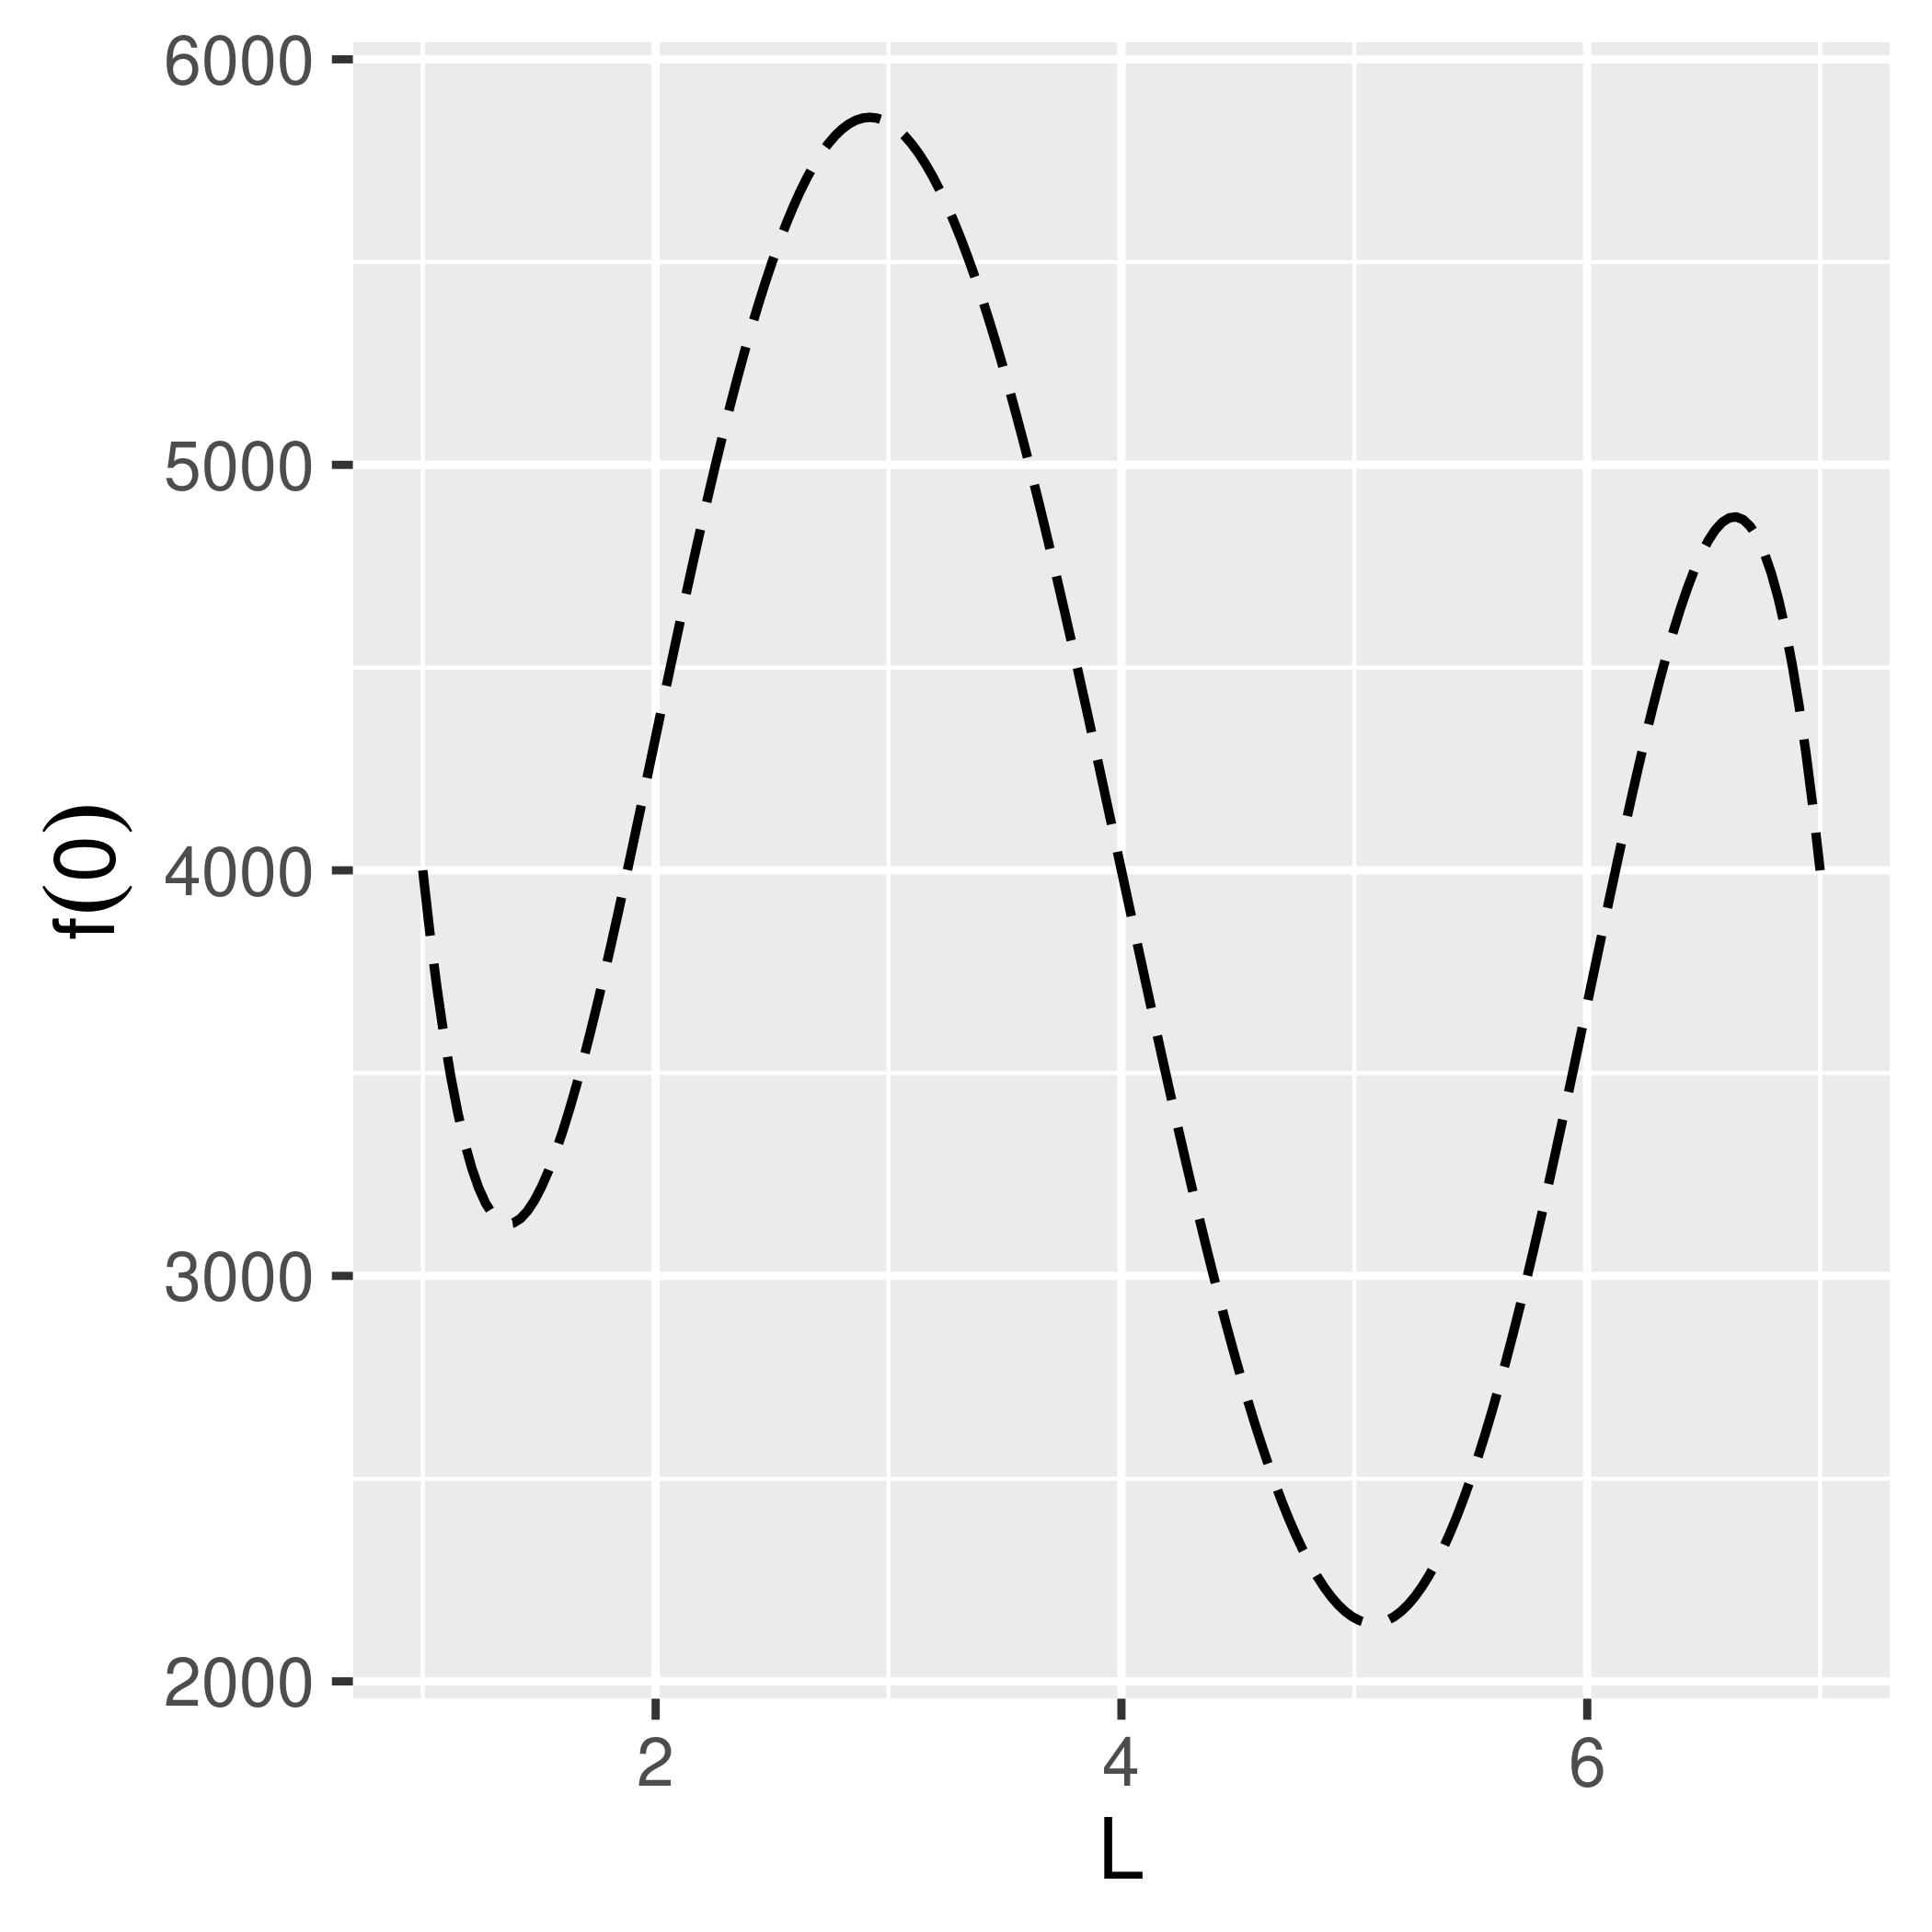
\includegraphics[width=0.6\textwidth]{initial_psd.png}
    \caption{ 
      {\small The initial condition $f(\ell, 0)$.}
    }
    \label{fig:initialpsd}
  \end{subfigure}
  \hfill
  \begin{subfigure}[b]{0.75\textwidth}
    \centering
    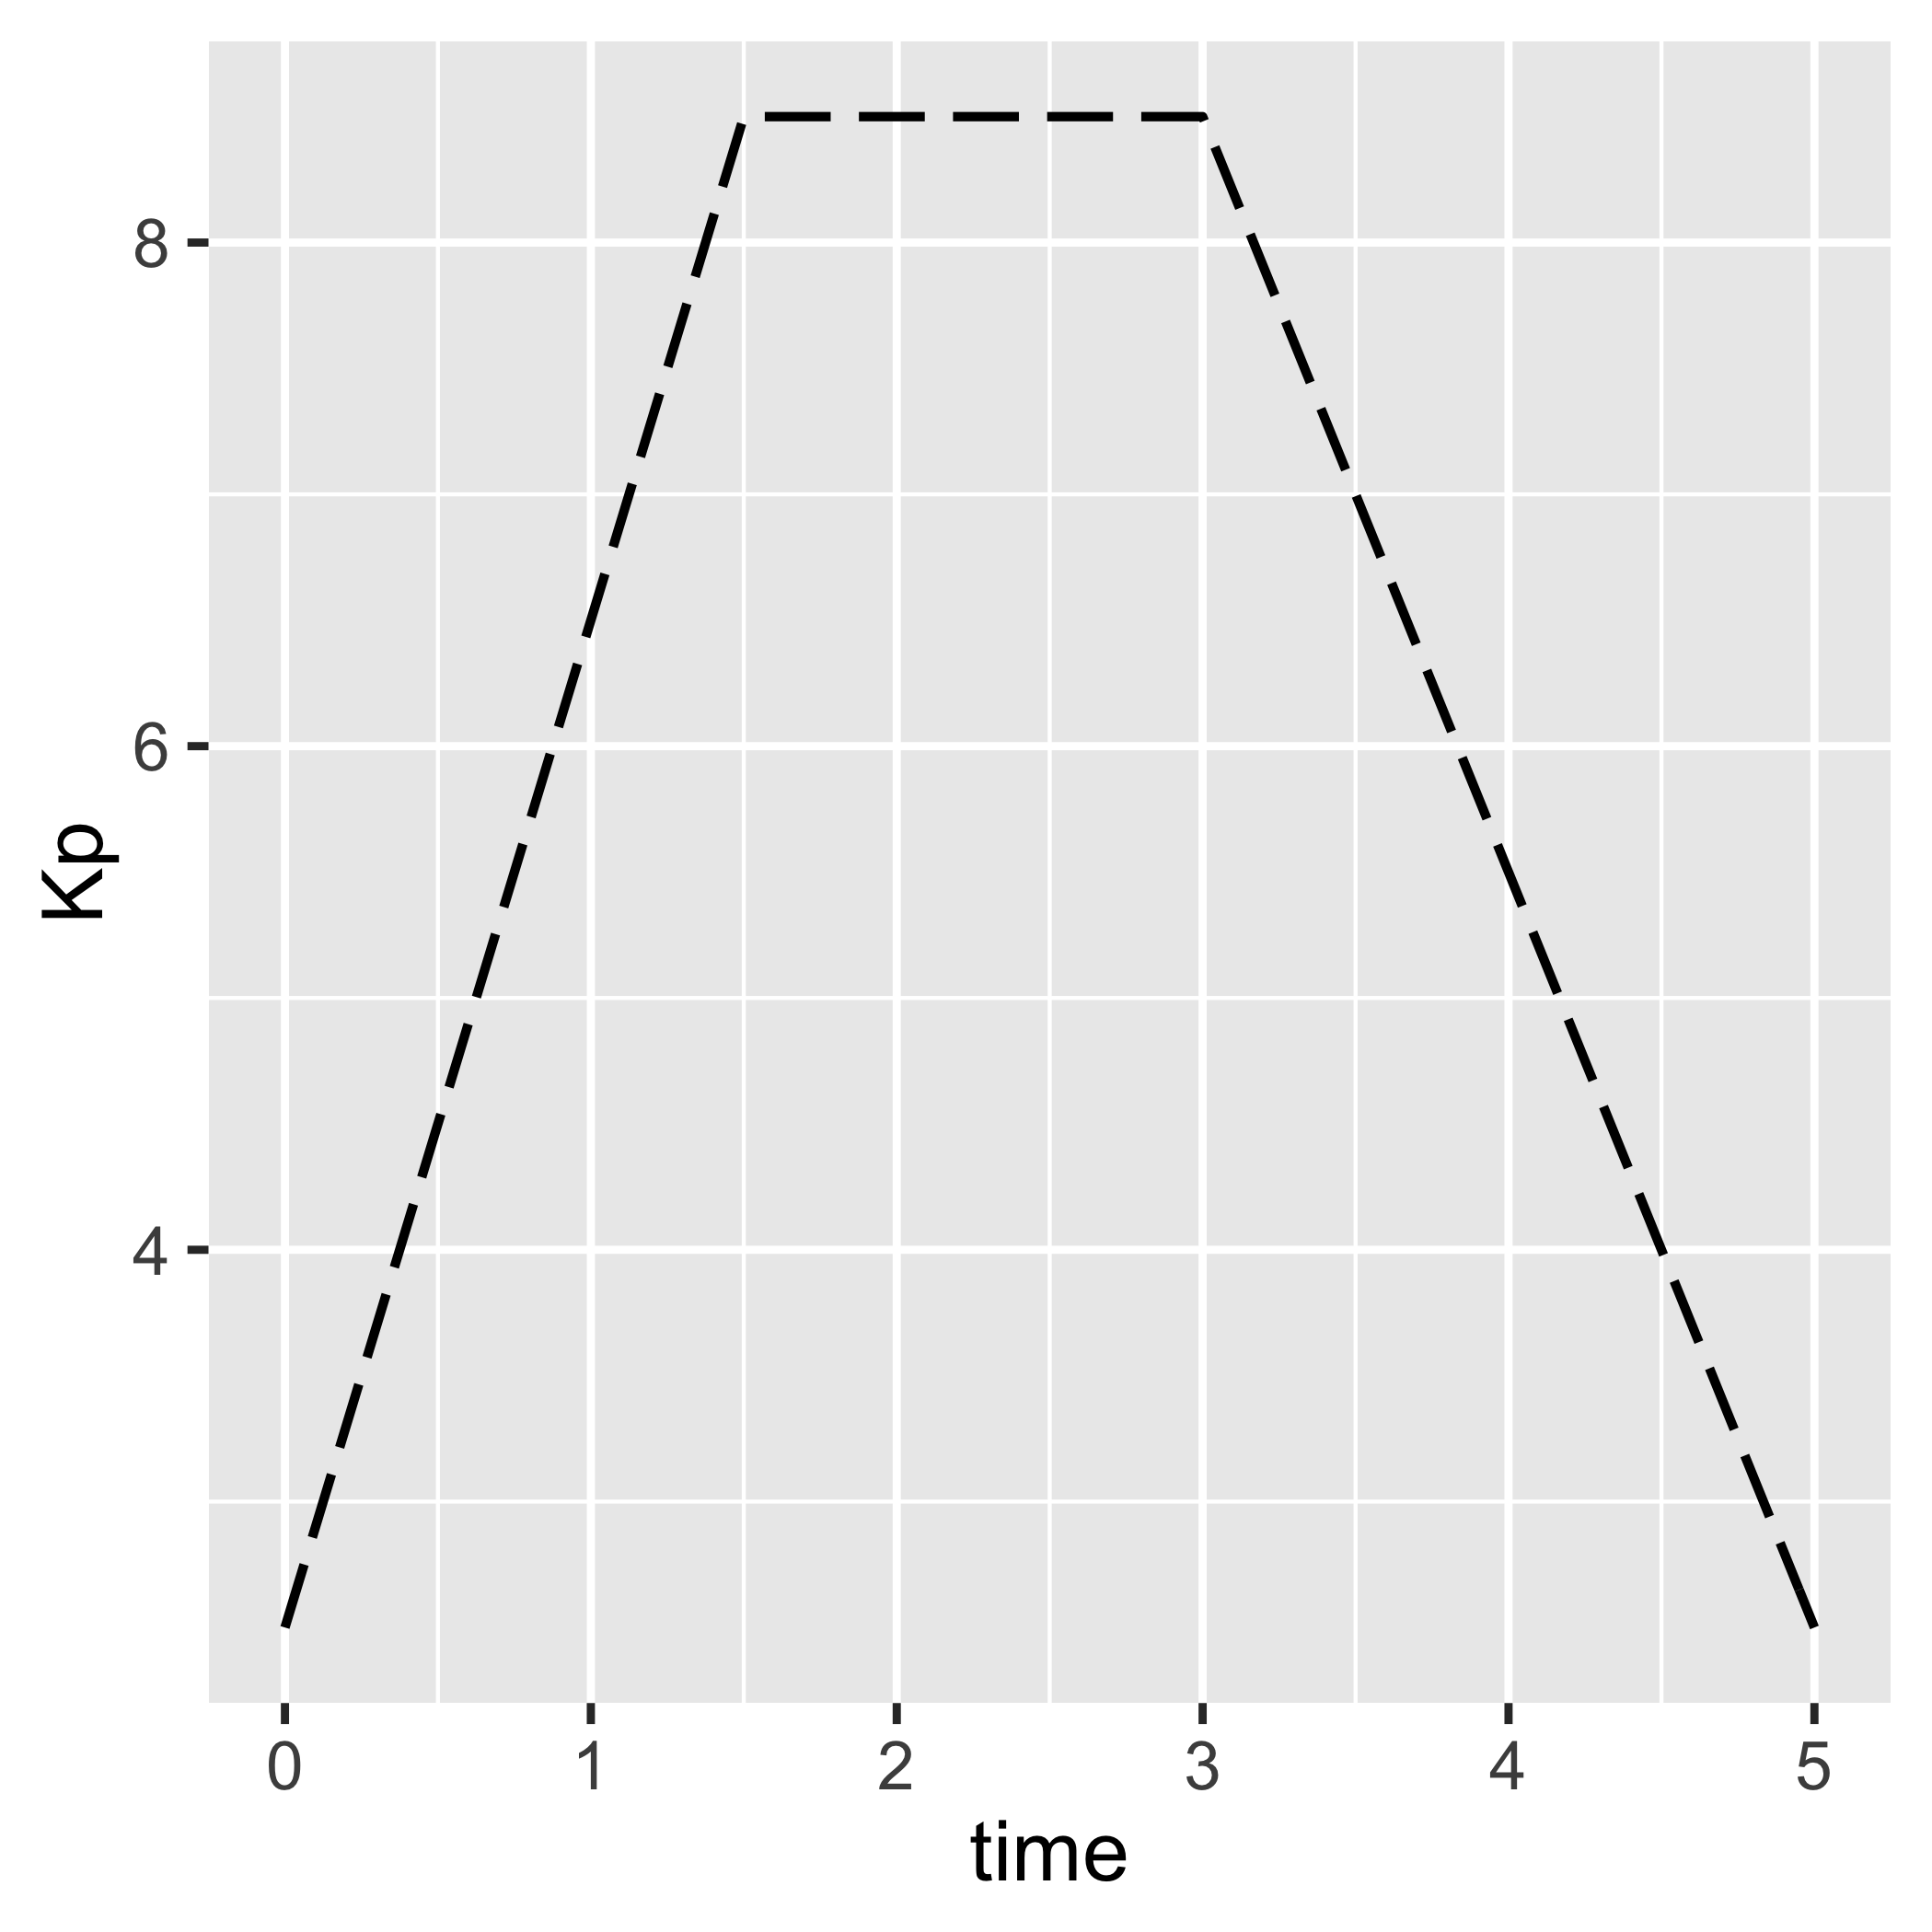
\includegraphics[width=0.6\textwidth]{kp_profile.png}
    \caption{
      {\small The time evolution of the Kp index.}
    }
    \label{fig:kpProfile}
  \end{subfigure}
  \caption{Synthetic data generation.}
\end{figure*}

 
The ground truth values of the radial diffusion parameters are listed in \cref{tab:ground-truth}.
%
The initial phase space density $f(t = 0)$ was chosen as follows (see \cref{fig:initialpsd}):
%
\begin{align*}
f(t = 0) &= 2000 + 500(T_{3}(\ell_*) - T_{5}(\ell_*)) \\
\ell_* &= 2\frac{\ell - \ell_{min}}{\ell_{max} - \ell_{min}} - 1 \ ,\\
\end{align*}
%
where $T_n(.)$ is the is the Chebyshev polynomial of degree $n$. The evolution of the Kp index was 
assumed to be an idealised version of a geomagnetic storm (see \cref{fig:kpProfile}) and 
defined as 
\[
  \mathrm{Kp}(t) = \left\{\begin{matrix}
    2.5 & 0 \leq t < 2\\ 
    2.5 + 4(t - 2d) & 2 \leq t < 3.5\\ 
    8.5 & 3.5 \leq  t < 5 \\ 
    23.5 - 3t & 5 \leq t < 7\\
    2.5 & t \geq 7\\ 
    \end{matrix}\right. \ .
\] 
%
The radial diffusion solver was run for domain limits $\ell \in [1, 7], t \in [0, 9]$ with $200$ 
bins in the spatial and $50$ bins in the temporal domains respectively. After the solution $f$ was 
computed, points was sub-sampled uniformly such that $250$ points lying in the interior of the 
domain, and $50$ points at the initial time step ($t = 0$) were selected. These observations were 
then perturbed by Gaussian noise to yield the final observation set $\mathcal{D}$ which was 
provided to the surrogate model $\hat{f}(x)$. The generated data set is plotted in 
\cref{fig:trainingDataQ}.


\begin{figure*}[!htb]
  \centering
  \begin{subfigure}[b]{0.75\textwidth}
    \centering
    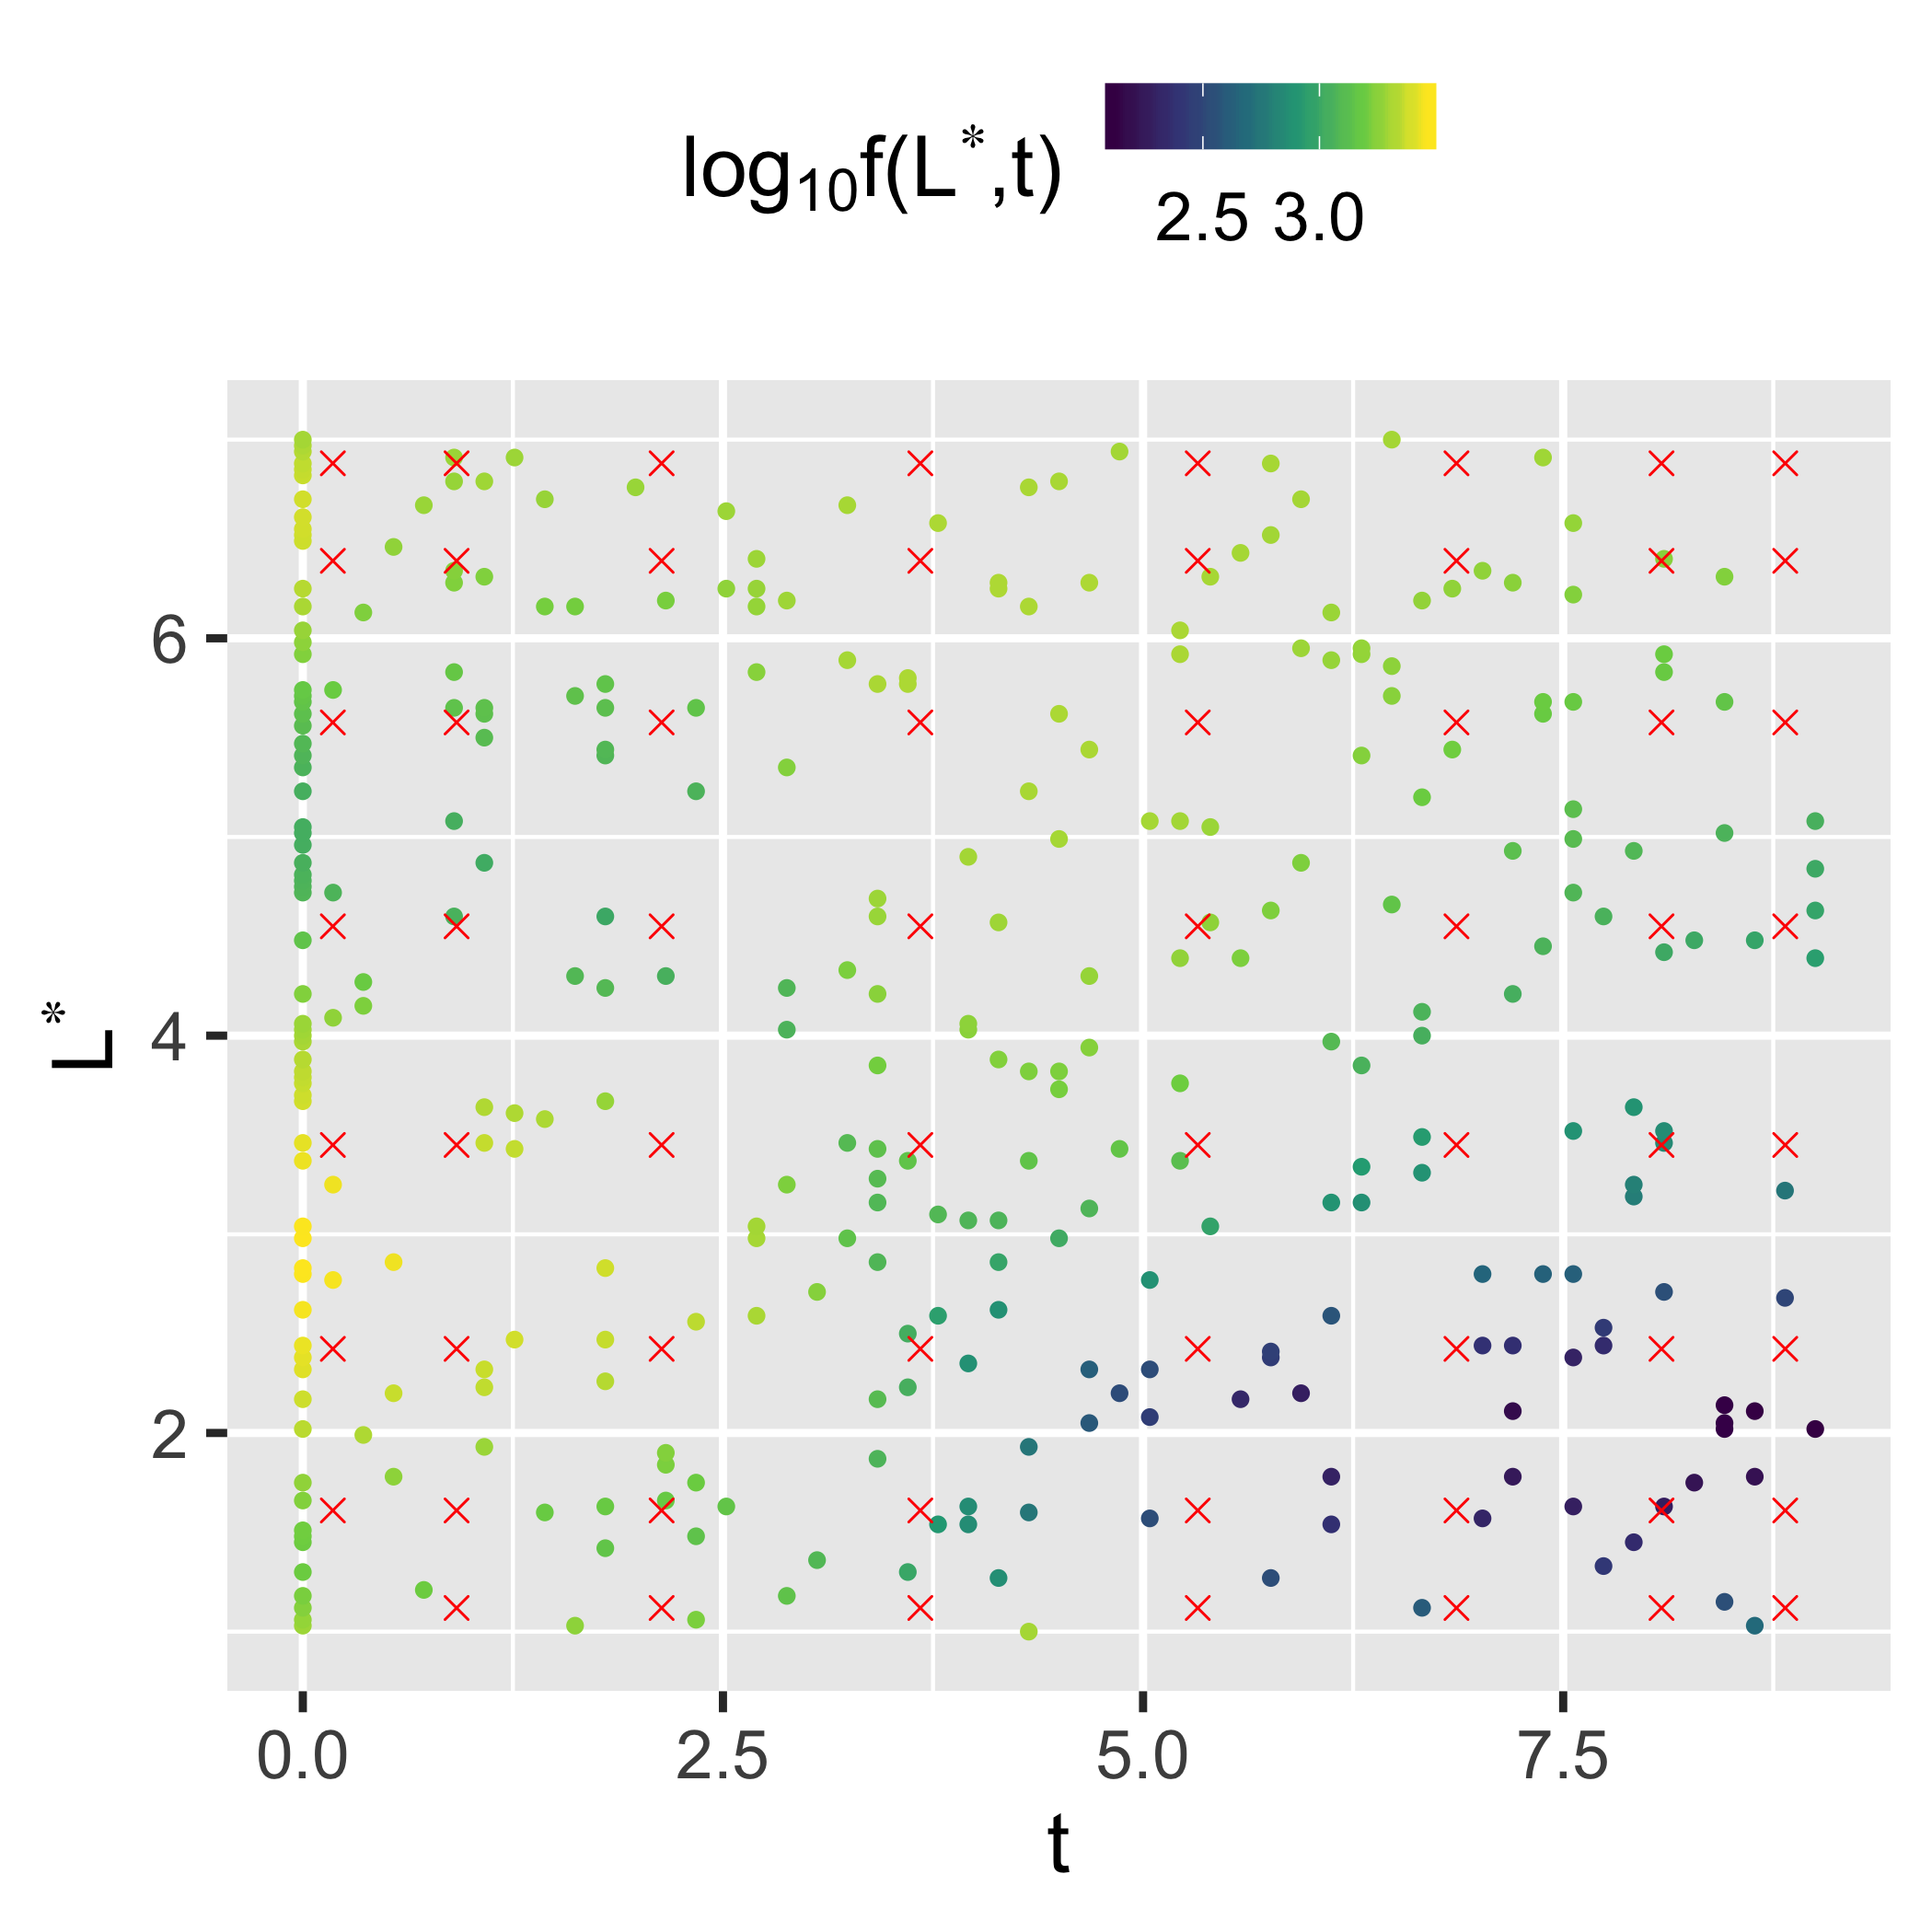
\includegraphics[width=0.6\textwidth]{data_and_design_points_Q.png}
    \caption{{\small 
      Synthetic data used in \cref{sec:syntheticDataQ}.
      Red crosses indicate colocation points chosen according to $8$ point Gauss-Legendre 
      quadrature in space and time. 
    }}
  \label{fig:trainingDataQ}
  \end{subfigure}
  \hfill
  \begin{subfigure}[b]{0.75\textwidth}
    \centering
    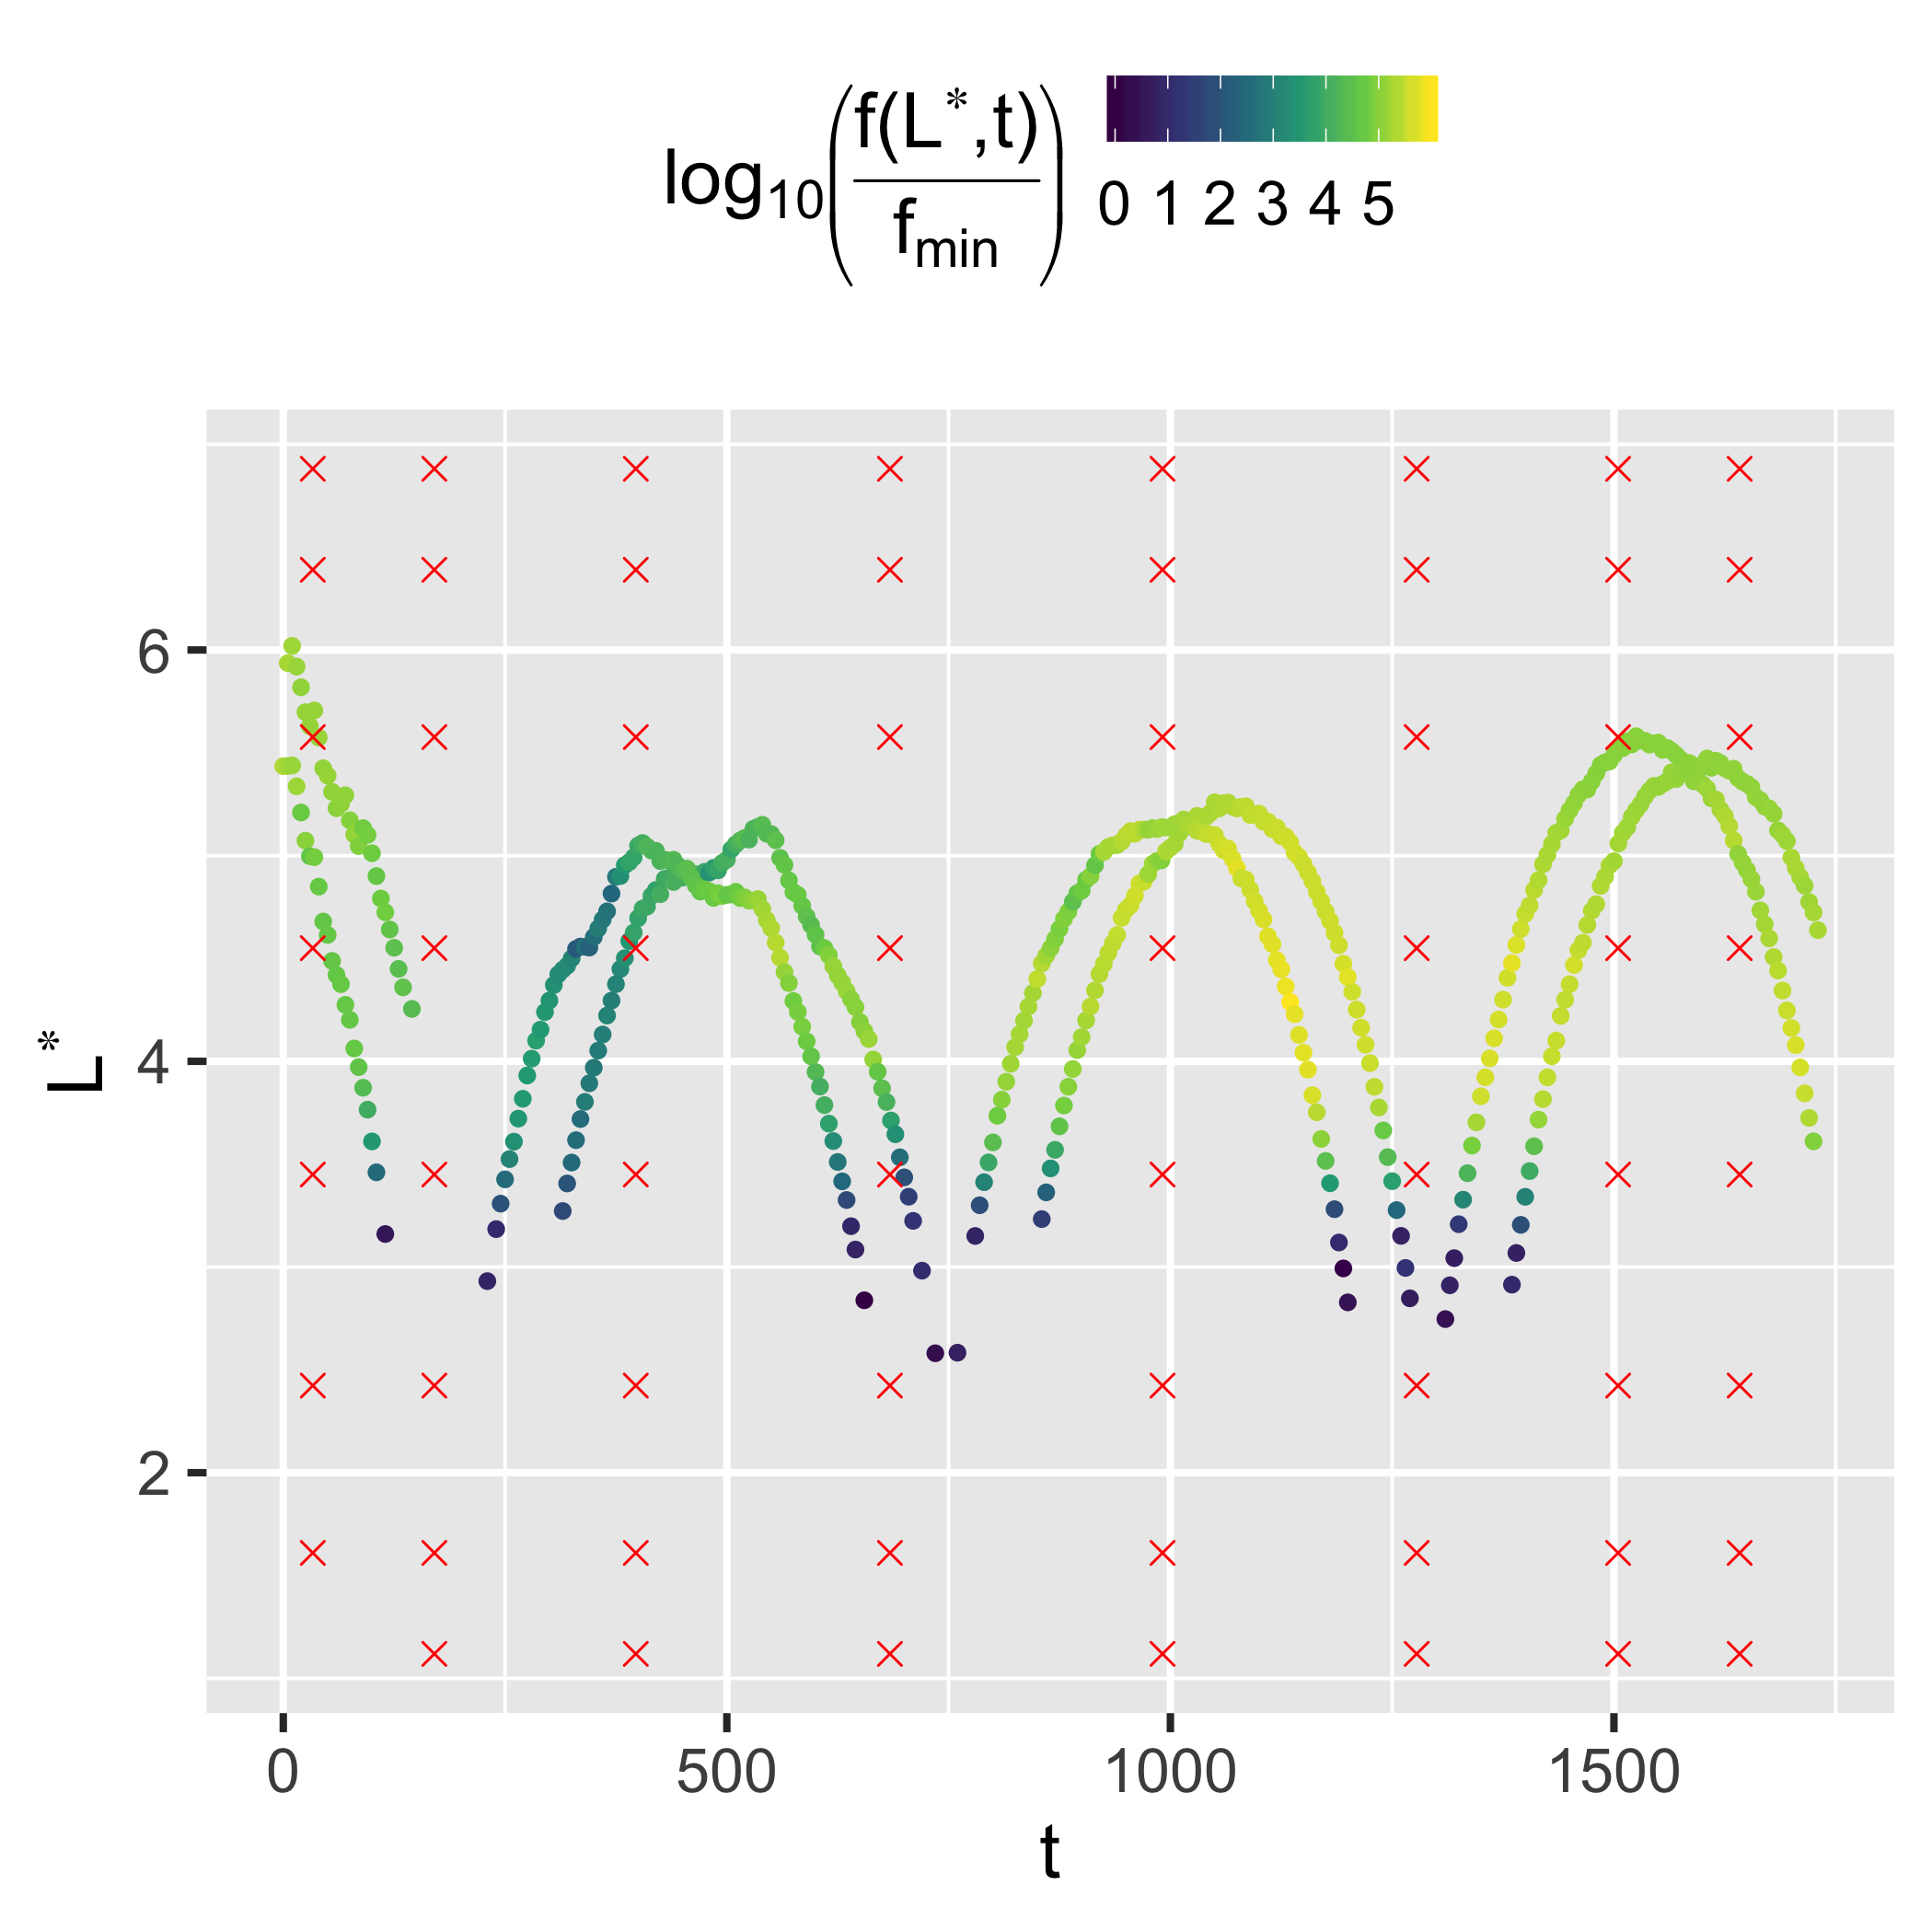
\includegraphics[width=0.6\textwidth]{data_and_design_points_van_allen.png}
    \caption{{\small 
      Van Allen probe data used in \cref{sec:vanAllenData}. Time is measured in minutes 
      from the starting point $6:00$ $17^{\text{th}}$ March $2013$. Red crosses indicate 
      colocation points chosen according to $8$ point Gauss-Legendre quadrature in space and time.
    }}
    \label{fig:trainingDataVanAllen} 
  \end{subfigure} 
  \caption{Data sets used in the experiments.}
\end{figure*}

\subsection{Radiation Belt Data: Van Allen Probes}\label{sec:vanAllenData}

Van Allen probe data from the \emph{MagEIS} instrument for the time period ranging from 
$6:00$ $17^{\text{th}}$ March $2013$ to $11:00$ $18^{\text{th}}$ March $2013$ was extracted and 
used for performing inference over the parameters of $q(\ell, t)$. This particular period was 
chosen because active geomagnetic conditions occurred in it. \Cref{fig:trainingDataVanAllen} 
plots the Van Allen PSD data on a logarithmic scale. To avoid dealing with extremely small values, 
we use $\log_{10}\left( \frac{f(\ell, t)}{f_{min}} \right)$, the logarithm of the ratio of the PSD 
to its observed minimum value in the data. 

There are two differences which stand out between the van allen data set and the synthetic data 
used in \cref{sec:syntheticDataQ} above. Firstly, the synthetic data is randomly sampled 
while the Van Allen probe data is sampled along their orbits (there are two probes). Secondly, 
the synthetic data is has a larger density of observations in the space time domain as compared to 
the Van Allen data. These factors among others influence the uncertainties in the posterior 
inference, which is seen in \cref{sec:diffResults} below.  

\subsection{Results}\label{sec:diffResults}

\begin{figure*}[!htb]
  \centering
  \begin{subfigure}[b]{0.5\textwidth}
    \centering
    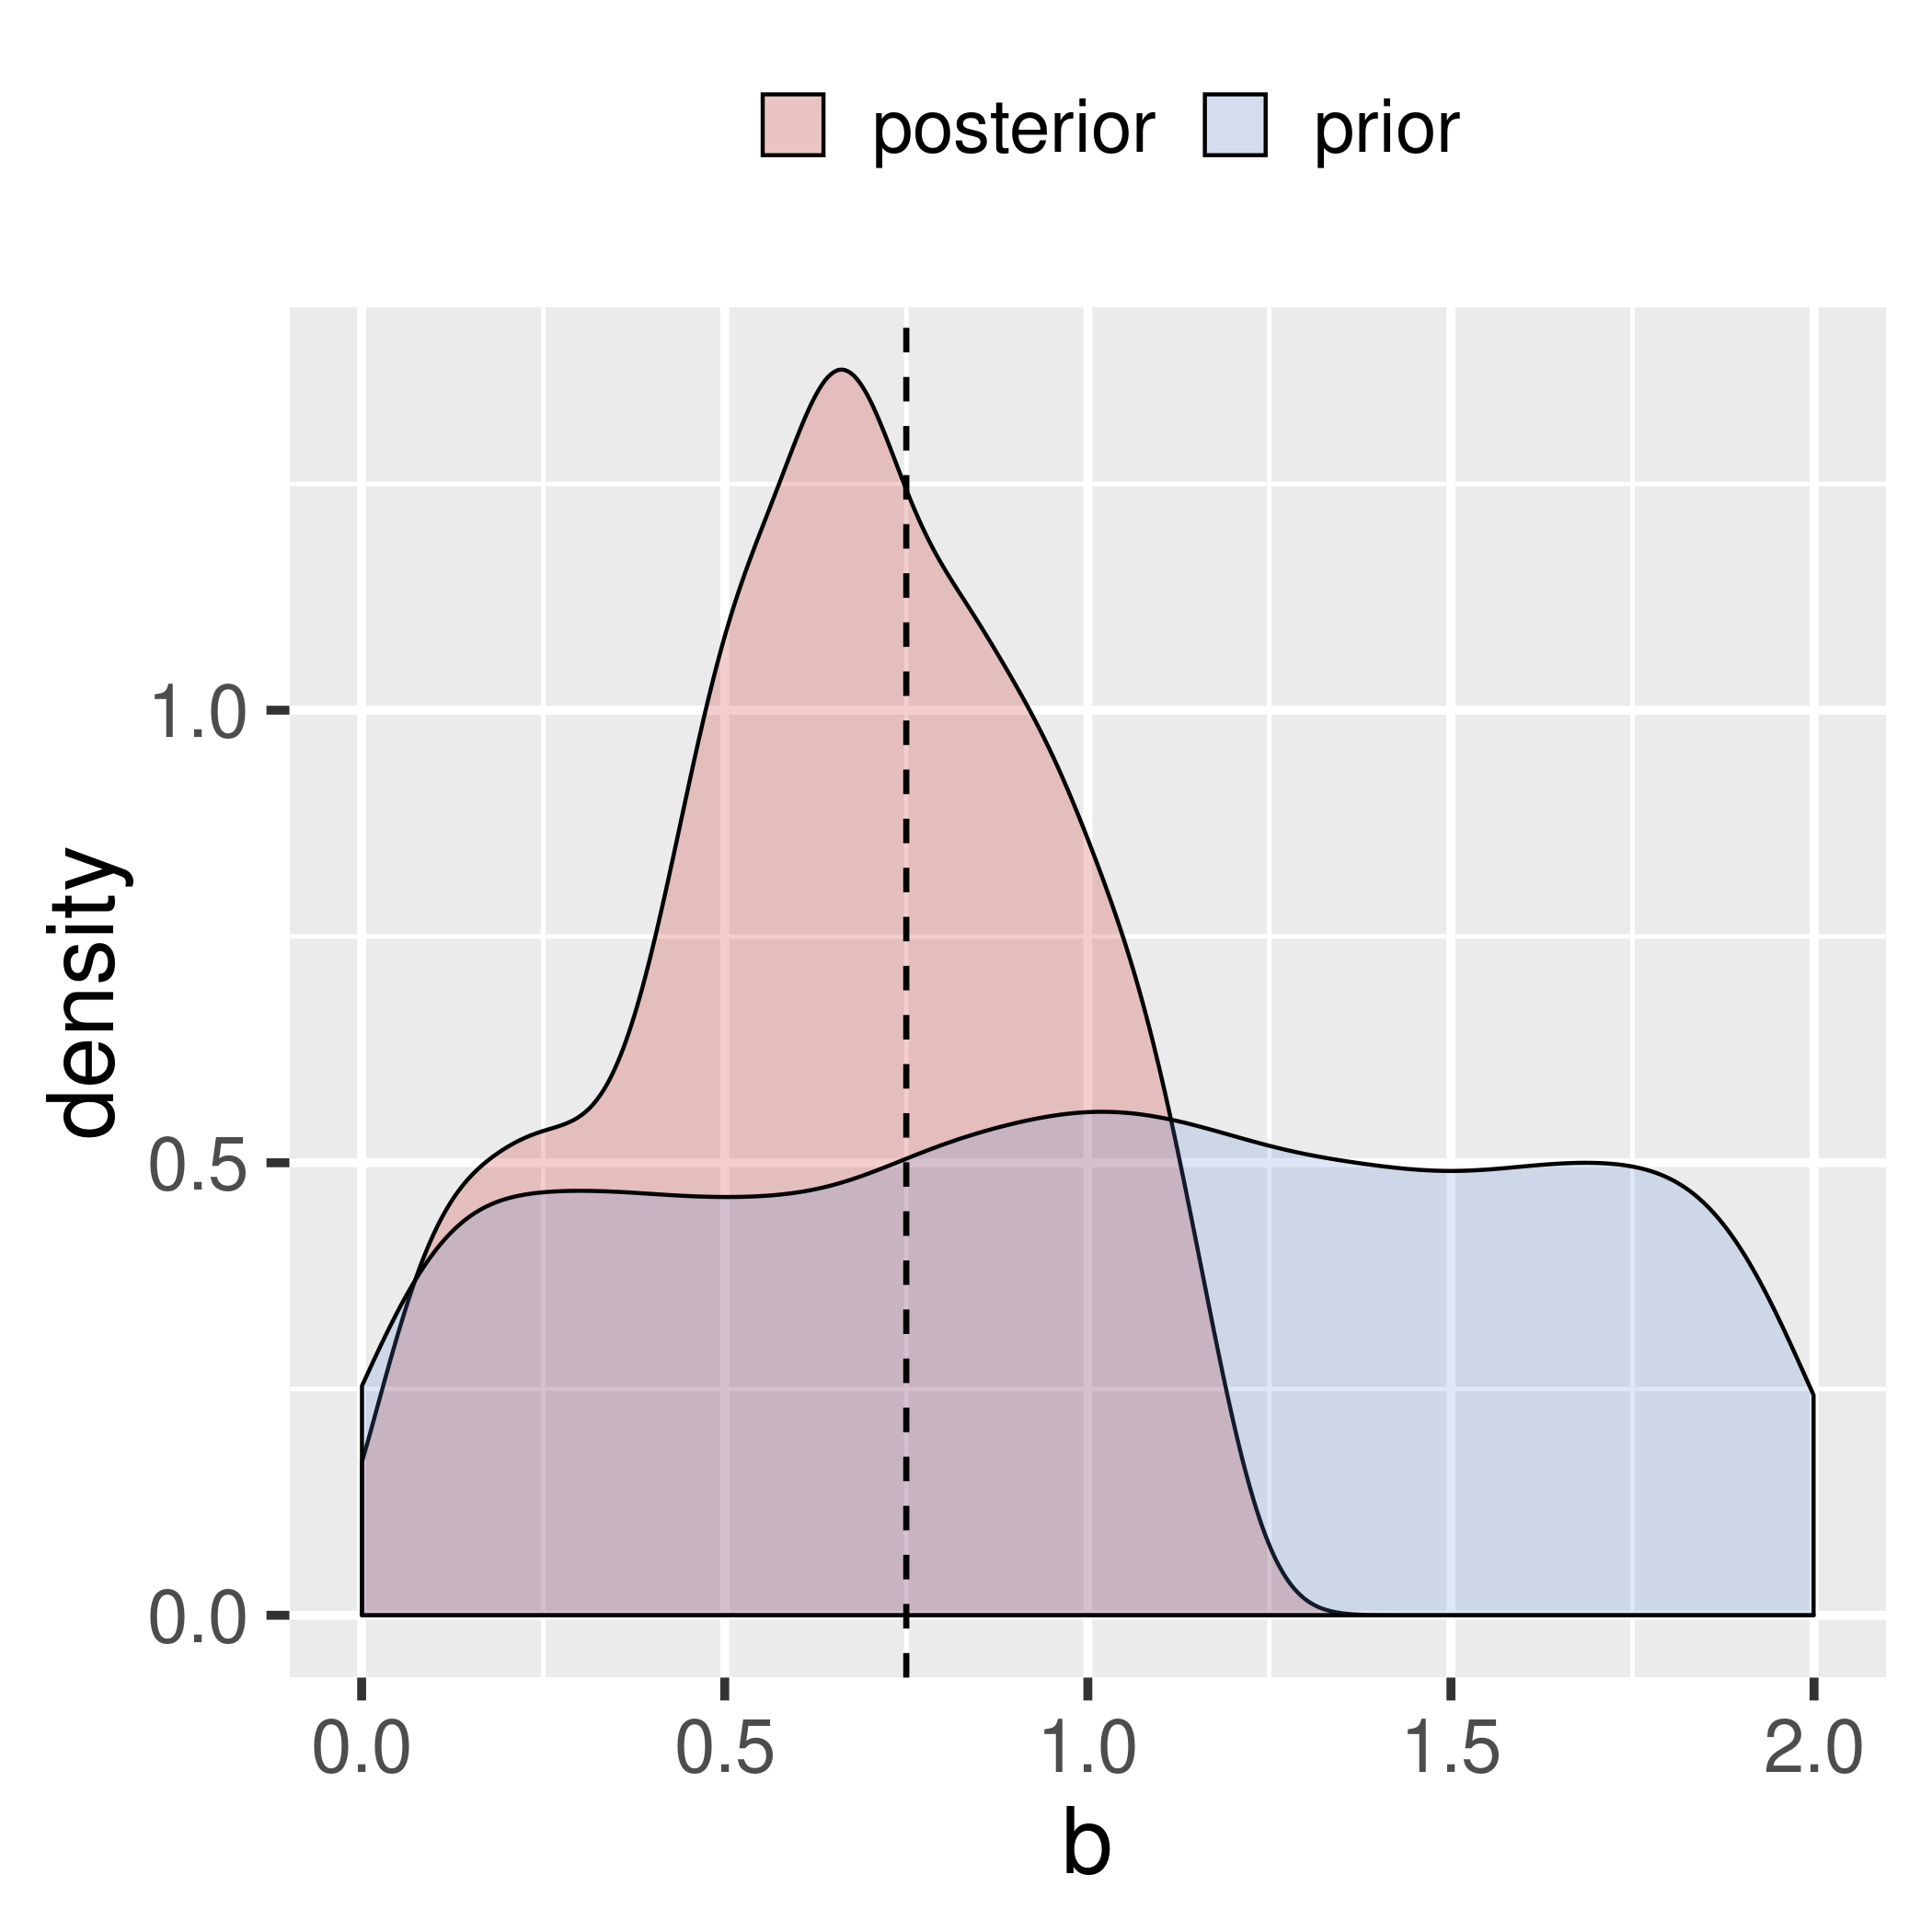
\includegraphics[width=0.6\textwidth]{density_Q_b.png}
    \caption{ {\small Parameter $b$}}
    \label{fig:qb}
  \end{subfigure}
  \hfill
  \begin{subfigure}[b]{0.5\textwidth}
    \centering
    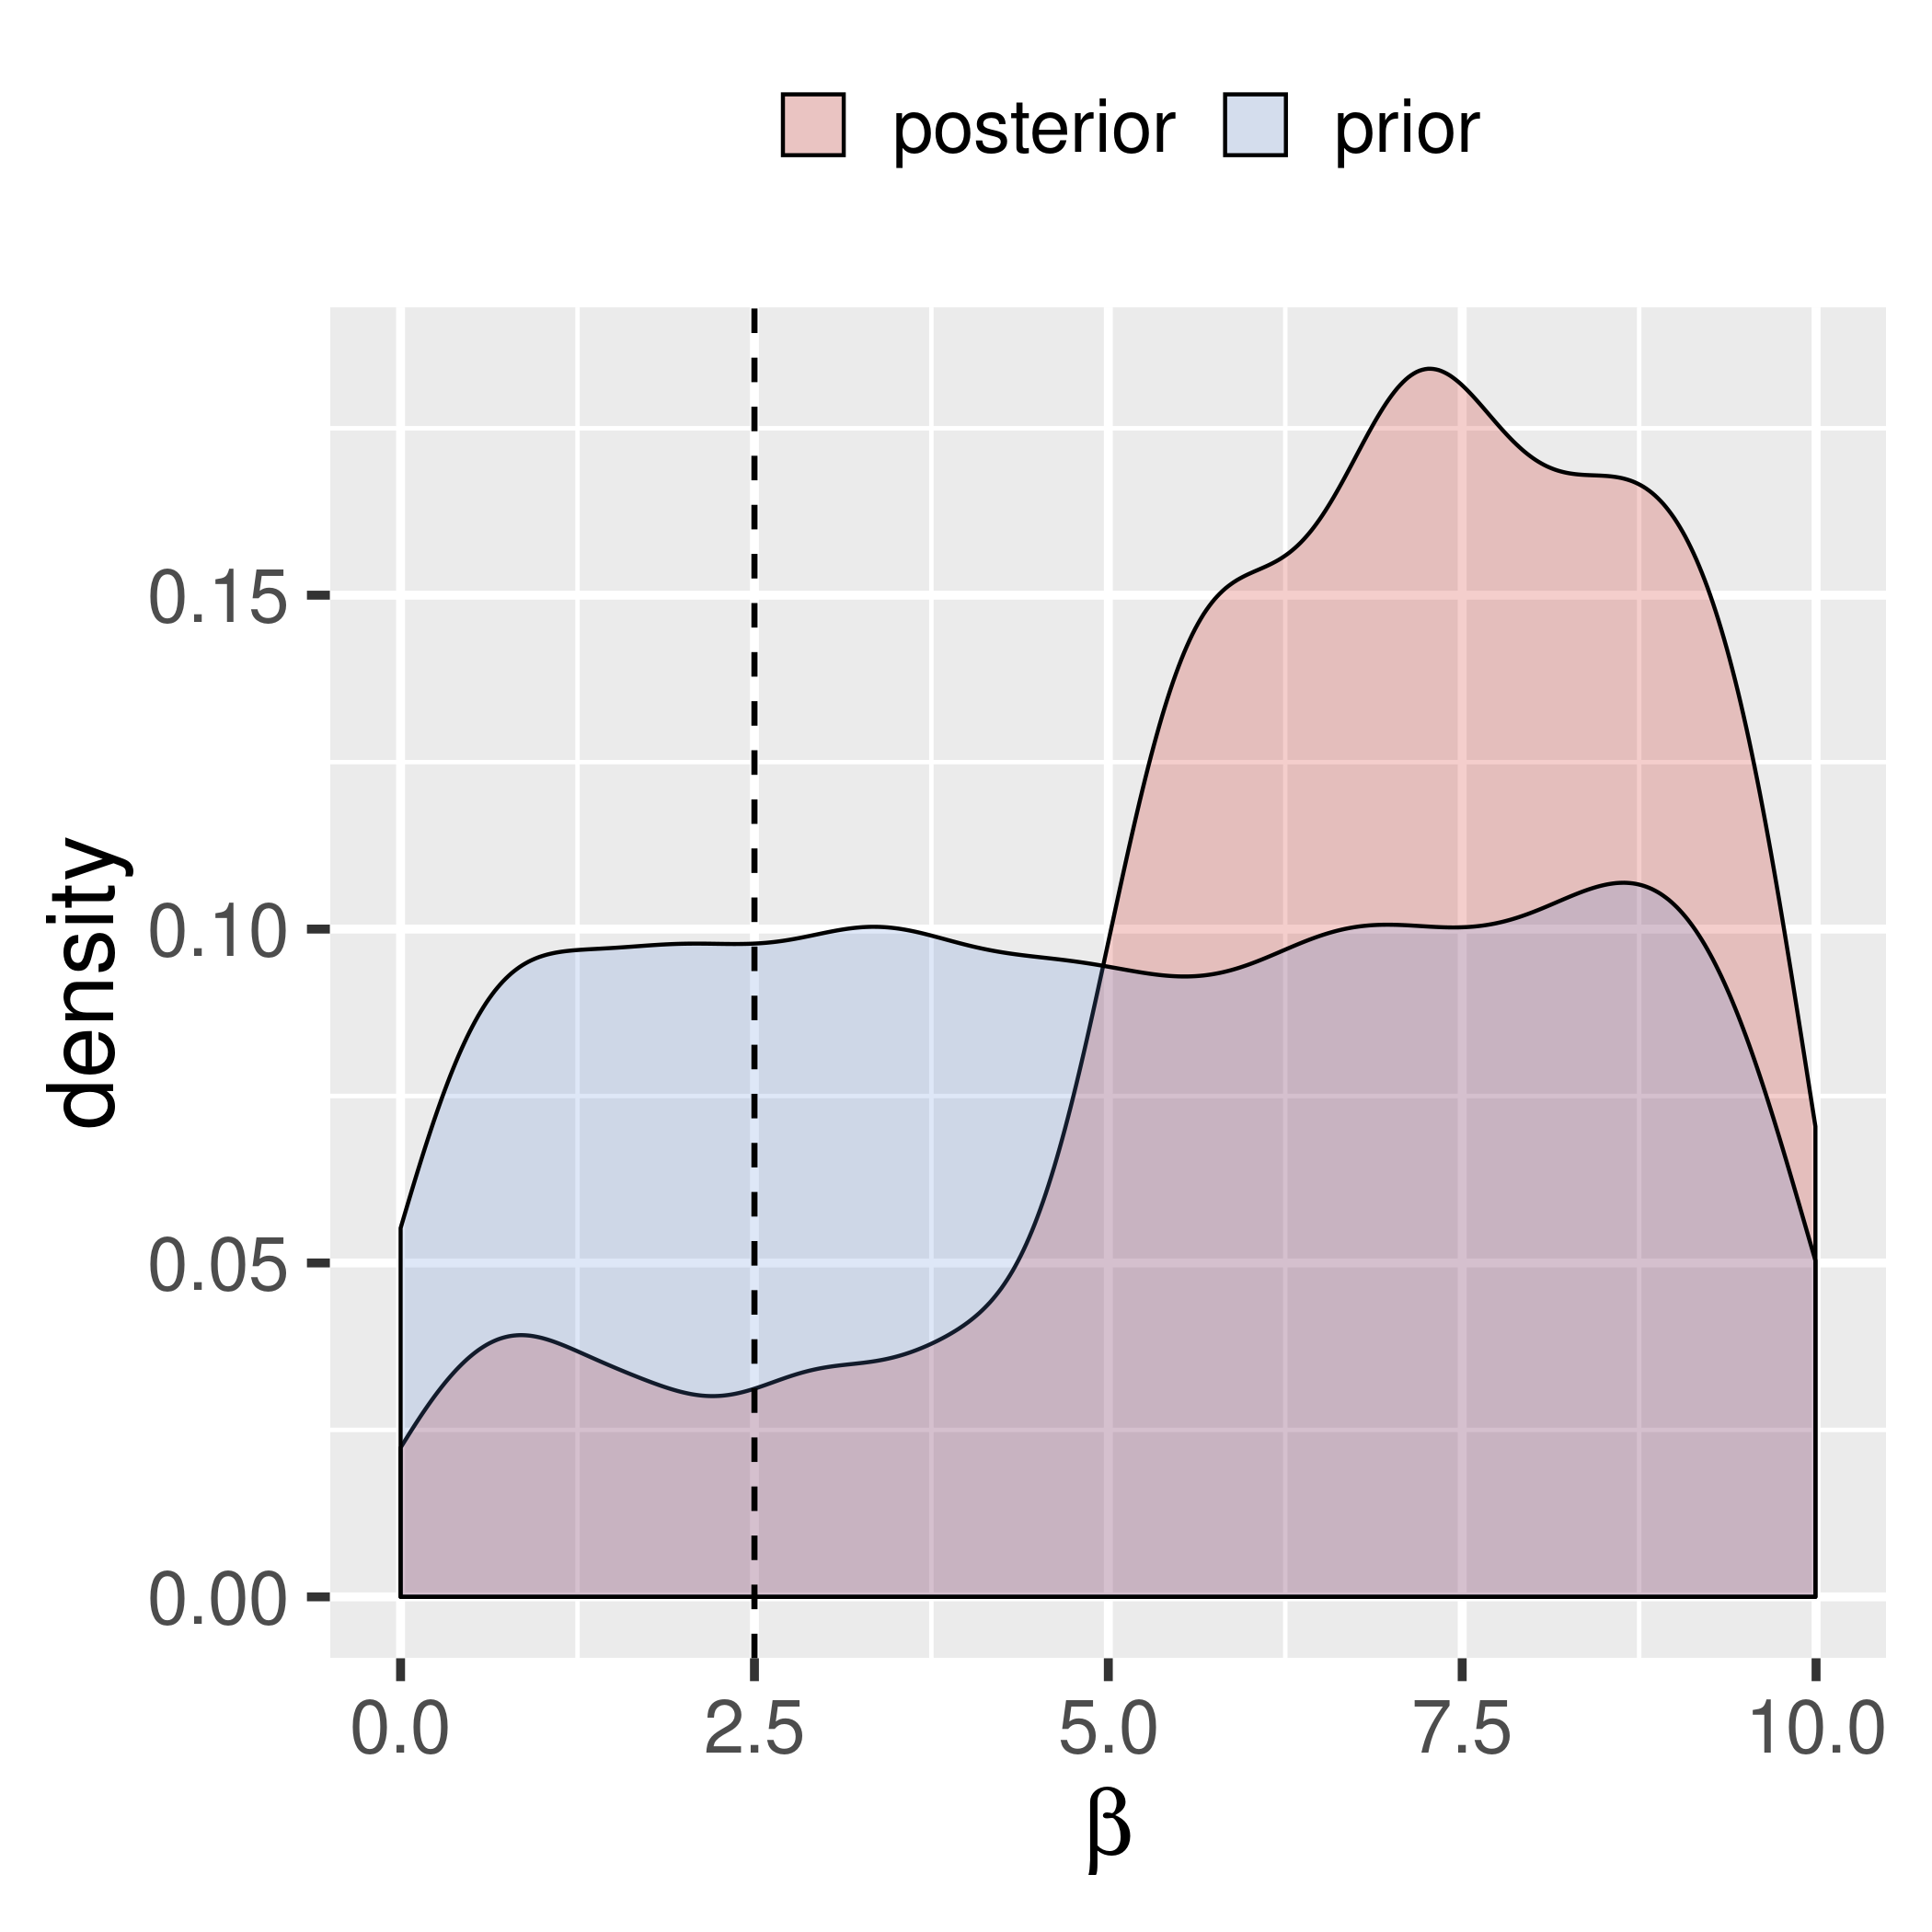
\includegraphics[width=0.6\textwidth]{density_Q_beta.png}
    \caption{{\small Parameter $\beta$}}
    \label{fig:qbeta}
  \end{subfigure}
  \hfill
  \begin{subfigure}[b]{0.5\textwidth}
    \centering
    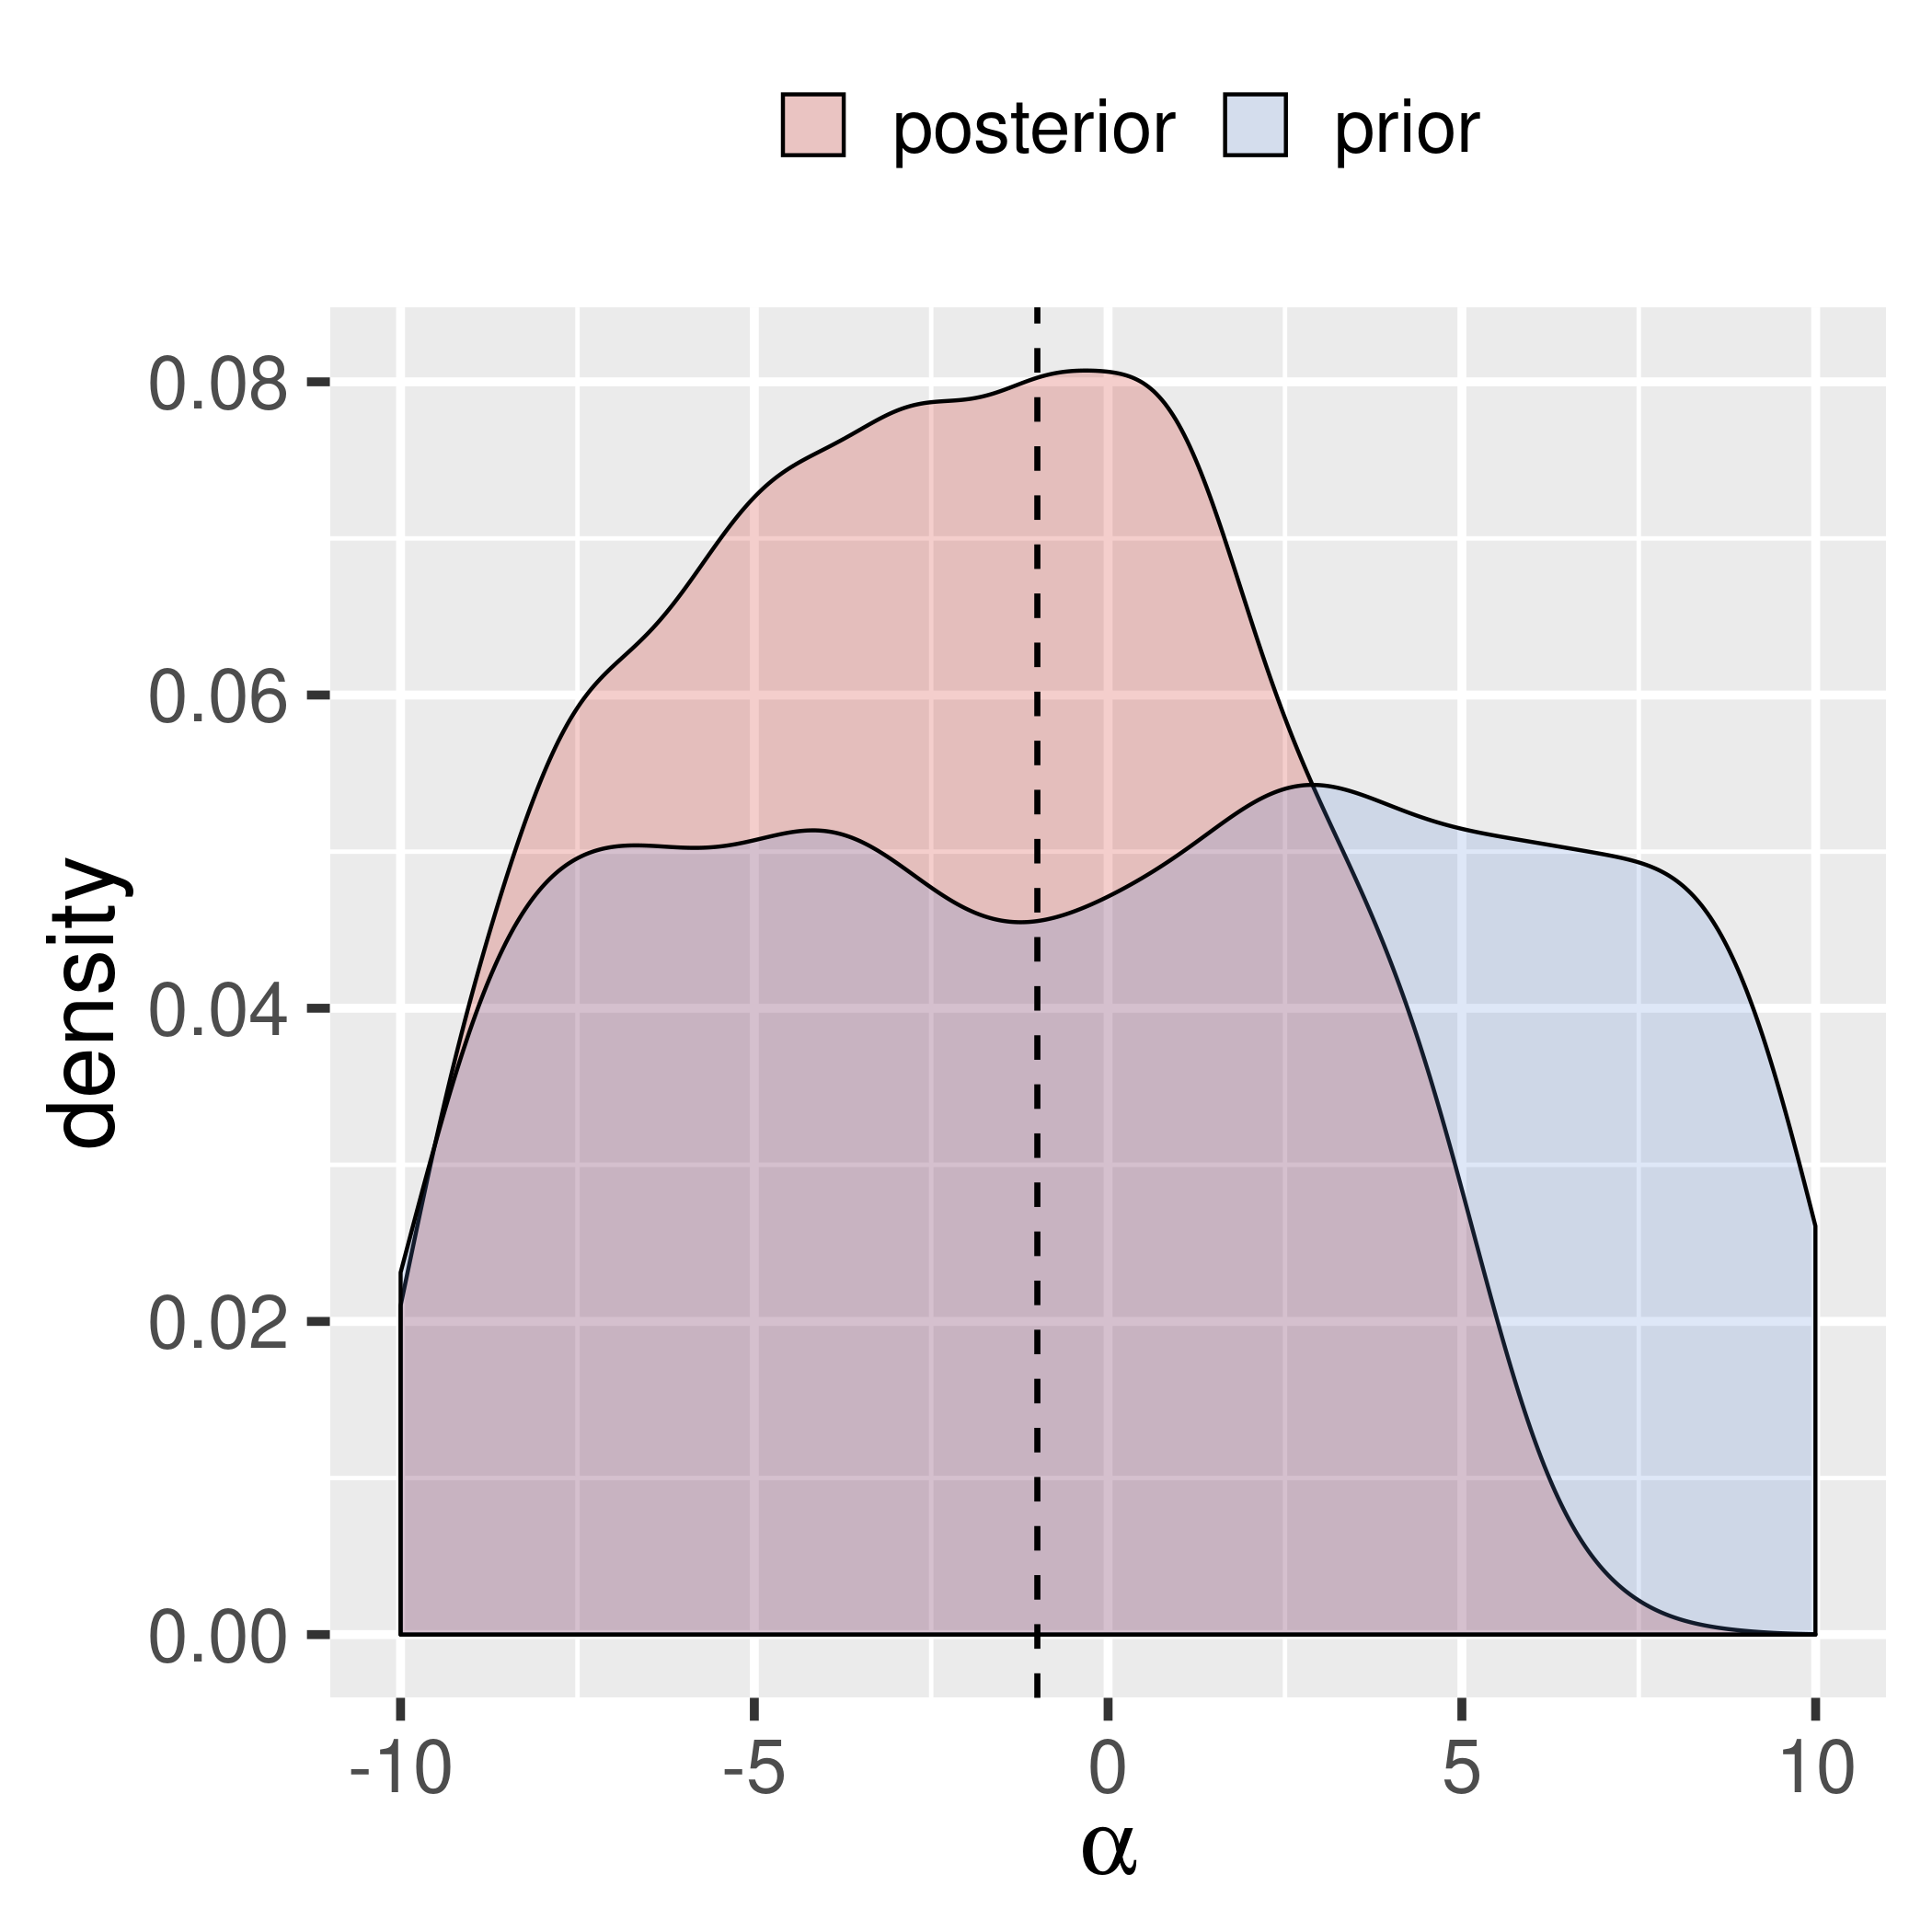
\includegraphics[width=0.6\textwidth]{density_Q_alpha.png}
    \caption{{\small Parameter $\alpha$}}
    \label{fig:qalpha}
  \end{subfigure}
  \caption{\textbf{Synthetic Data}: Comparing prior and posterior densities for 
  parameters of $q(\ell, t)$, the black dotted line indicates the ground truth.}  
\end{figure*}

\begin{figure*}[!htb]
  \centering
  \begin{subfigure}[b]{0.75\textwidth}
    \centering
    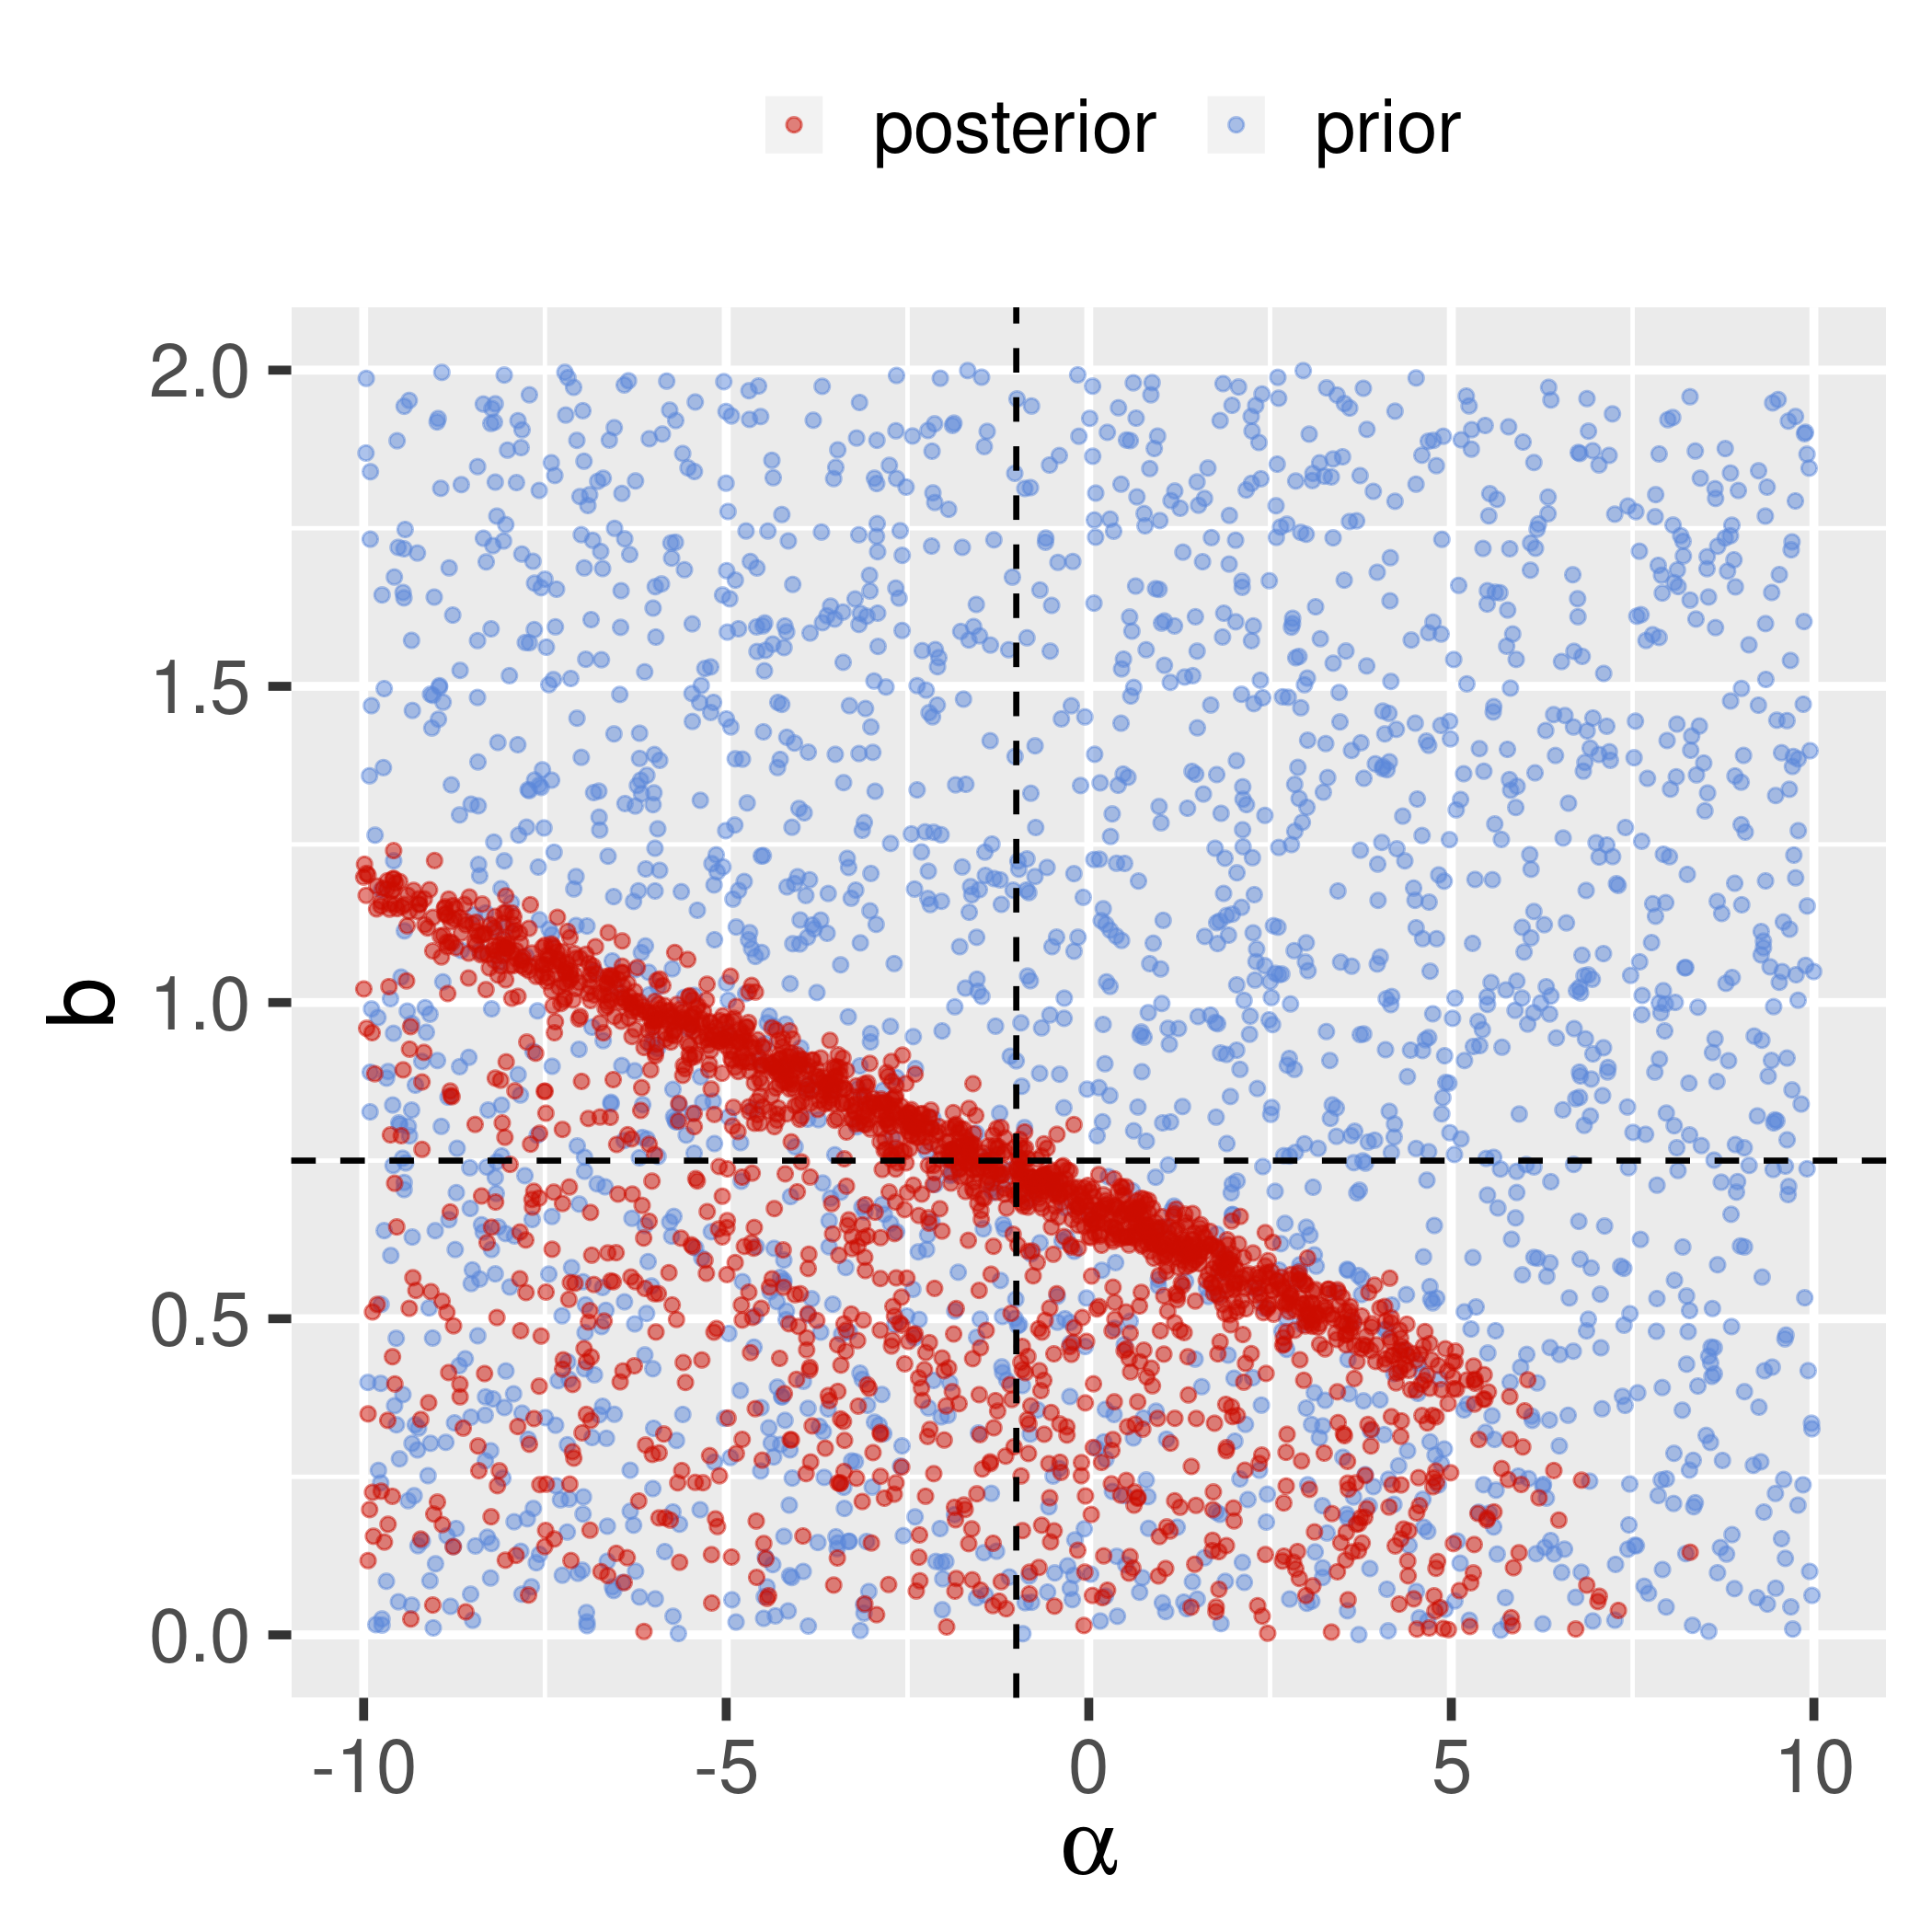
\includegraphics[width=0.6\textwidth]{prior_posterior_scatter_Q_alpha_b.png}
    \caption{{\small Scatter chart: $\alpha$ versus $b$.}}
    \label{fig:alphavsb}
  \end{subfigure}
  \hfill
  \begin{subfigure}[b]{0.75\textwidth}
    \centering
    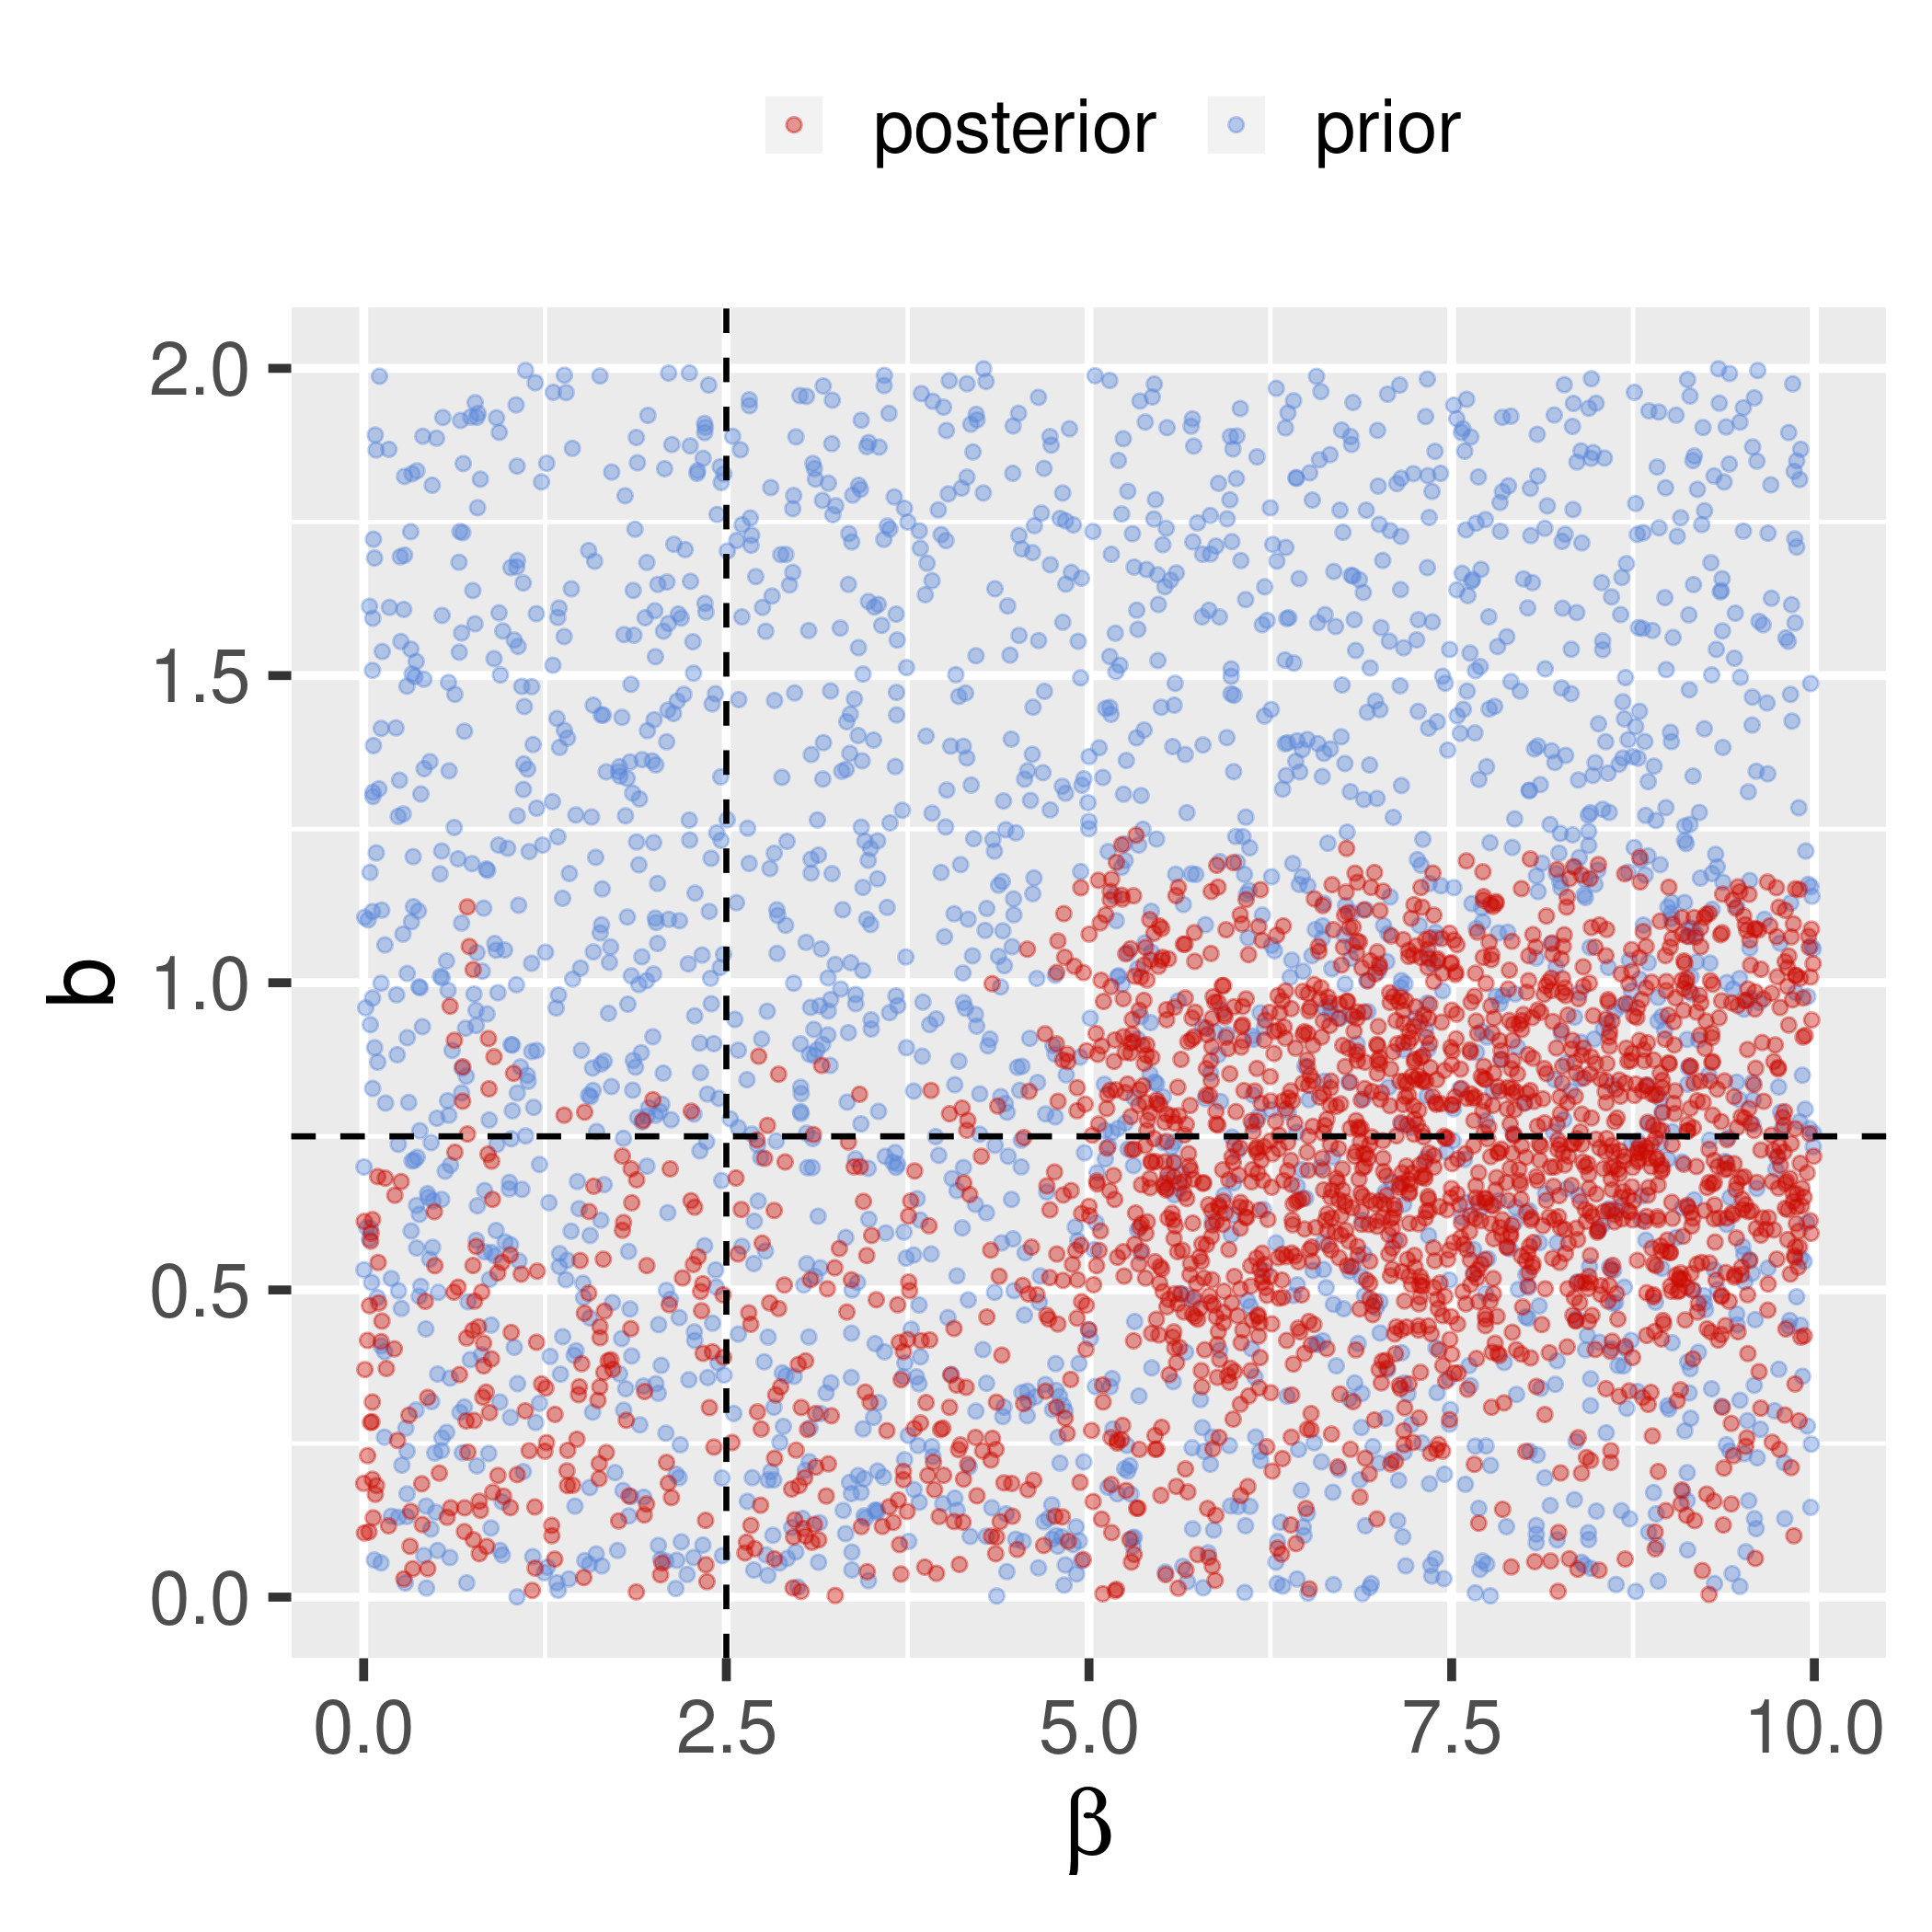
\includegraphics[width=0.6\textwidth]{prior_posterior_scatter_Q_beta_b.png}
    \caption{{\small Scatter chart: $\beta$ versus $b$.}}
    \label{fig:betavsb}
  \end{subfigure}
  \caption{\textbf{Synthetic Data}: Prior and posterior samples drawn 
  from parameters of $q(\ell, t)$.}
\end{figure*}

\subsubsection*{Synthetic Problem}

For the synthetic problem, the inferred posterior distribution for parameters of the particle 
injection rate $q(\ell, t)$ are shown in \cref{fig:qb,fig:qbeta,fig:qalpha}. We see that the 
marginal posterior distributions of $b$ and $\alpha$ have high probability density near the ground 
truth. 

The scatter charts in \cref{fig:alphavsb,fig:betavsb} help us to identify regions in the 
parameter space to which our model assigns high probability. From the scatter plot in 
\cref{fig:alphavsb}, we see a clear negative correlation between $\alpha$ and $b$. This negative 
correlation is a natural consequence of the parametrization of $q(\ell, t)$ in \cref{eq:q}. When 
$\alpha$ is increased, $b$ must appropriately decreased if one is to explain the PSD observations. 
Examining the dependence between $\alpha$ and $b$ in \cref{fig:alphavsb}, one can make the 
interpretation that along the red linear region corresponding to high posterior probability, all 
values of $\alpha$ and $b$ can explain the PSD observations with similar likelihood. We also 
observe that the density of posterior samples is greater below the red linear region as compared to 
above it.

From \cref{fig:qbeta,fig:betavsb}, we observe that the model doesn't identify the parameter 
$\beta$. Its posterior probability distribution does not have significantly reduced uncertainty 
compared to its prior. The differences in the inference results between parameters $\alpha, b$, and 
$\beta$ can be attributed to the vast differences in the sensitivity of the radial diffusion 
solution to $\alpha$, $b$, and $\beta$. The interested reader can refer to 
\cref{app:psdSensitivity} for an introduction to the sensitivity analysis of partial differential 
equations and its application to the radial diffusion system.     

\subsubsection*{Radiation Belt Particle Injection}

From \cref{fig:qbvanAllen,fig:qbetavanAllen,fig:qalphavanAllen}, we see that the posterior 
probabilities for $b$, $\beta$, and $\alpha$ approximately peak at $0.64$, $4.8$, and $-5$ 
respectively. In \cref{fig:alphavsbvanAllen}, we see a negative correlation between $\alpha$ and 
$b$ similar to what was observed in \cref{fig:alphavsb}.

Although the posterior distributions are not uninformative like the uniform priors, they have 
significantly greater uncertainty as compared to the results of the synthetic problem. This is 
because of two principal causes.
\begin{enumerate}
  \item \emph{Data sparsity}: The radiation belt data is sparsely sampled as compared to the 
        synthetic data.
  \item \emph{Forward model inadequacy}: The radial diffusion PDE is a simplified model for the 
        dynamics of the radiation belt. This inadequacy of the forward model can have a strong 
        influence in parameter uncertainties. 
\end{enumerate}


\section{Conclusions}

In this chapter, we proposed a surrogate model for the phase space density of particles in the 
radiation belt, and we presented a method for applying it on the Bayesian inverse problem of 
quantifying uncertainties in parameters of the simplified radial diffusion model for radiation 
belt dynamics. 

We used our model to perform inference of radial diffusion source term parameters. For this 
purpose, we tested it on two data sets: 
\begin{enumerate}
  \item synthetically generated phase space density data and 
  \item in-situ measurements taken by the Van Allen probes. 
\end{enumerate}
%
The model enabled the identification of regions in the parameter space which have a high 
probability of producing phase space density values which close to the observations.

The strength of the proposed method is the ability to quantify the uncertainty in the parameters of 
a physical system, from a sparse set of observations. Due to the formulation of the surrogate 
optimisation in its dual form, it allows the inference to scale well with respect to high 
dimensional basis function expansions. The method can be applied for parameter inference of 
linear partial differential equations and warrants further research in its improvement.

\begin{figure*}[!htb]
  \centering
  \begin{subfigure}[b]{0.5\textwidth}
    \centering
    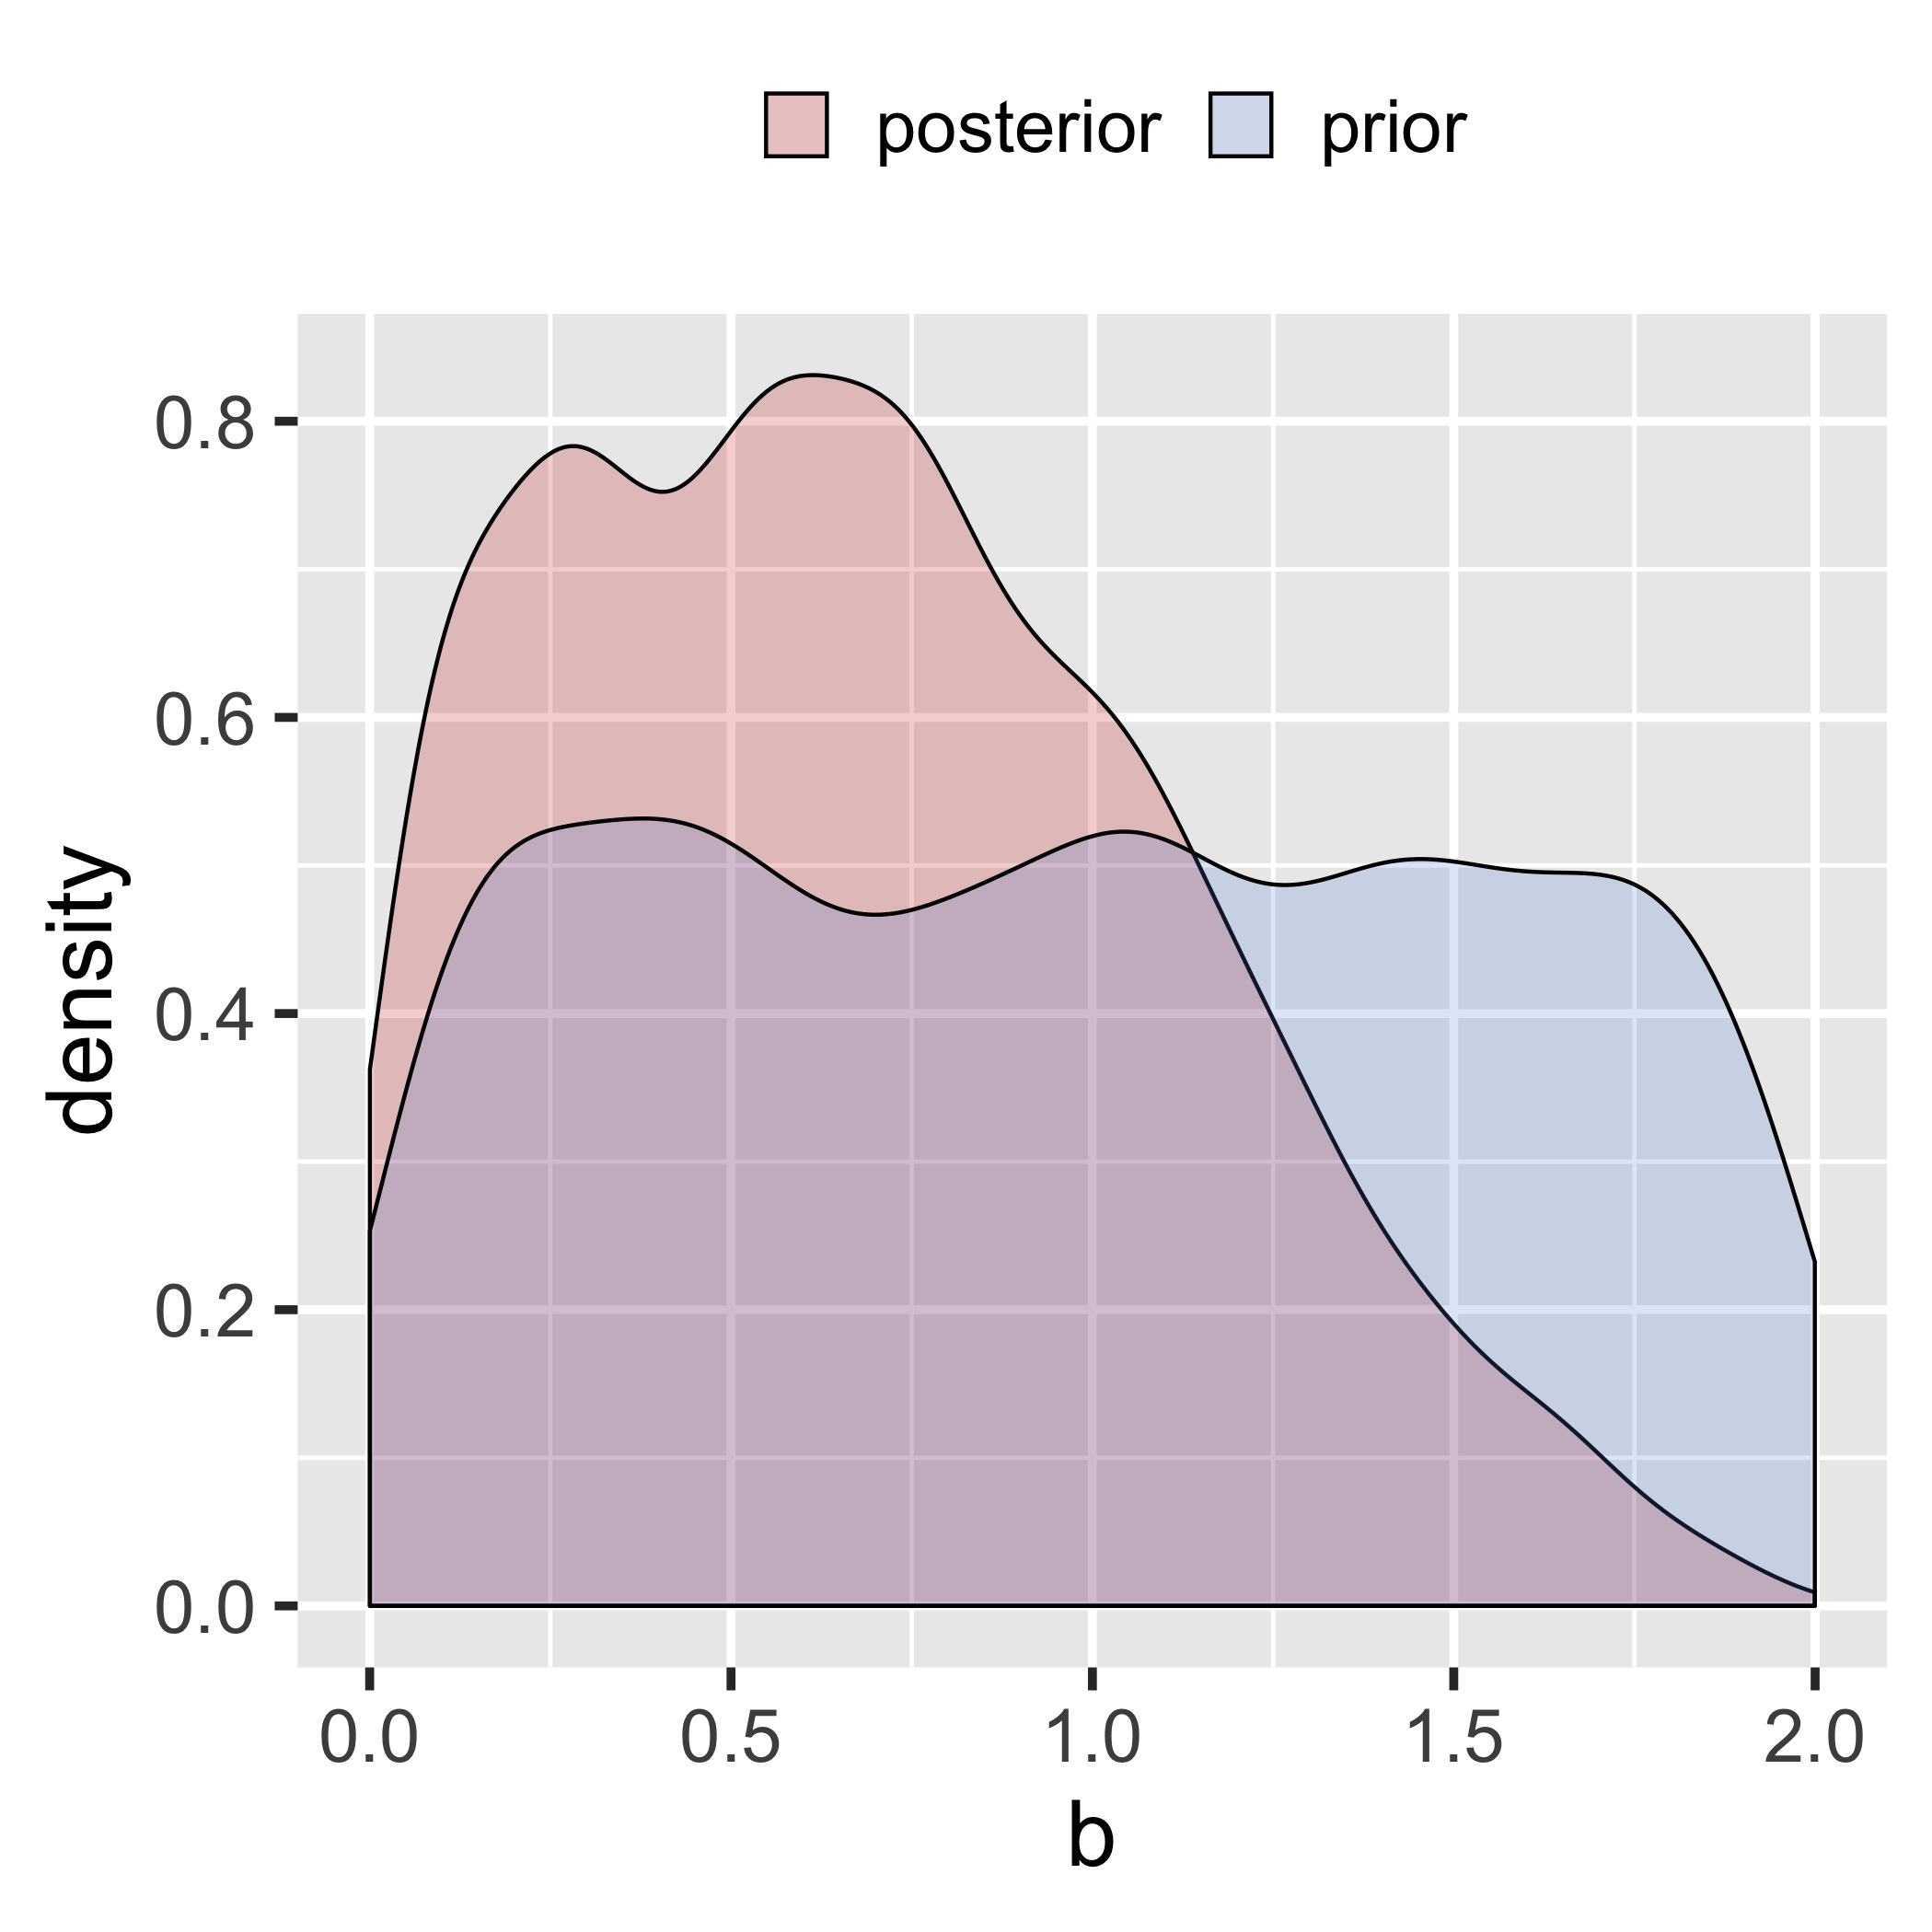
\includegraphics[width=0.6\textwidth]{van_allen_density_Q_b.png}
    \caption{{\small Parameter $b$}}
    \label{fig:qbvanAllen}
  \end{subfigure}
  \hfill
  \begin{subfigure}[b]{0.5\textwidth}
    \centering
    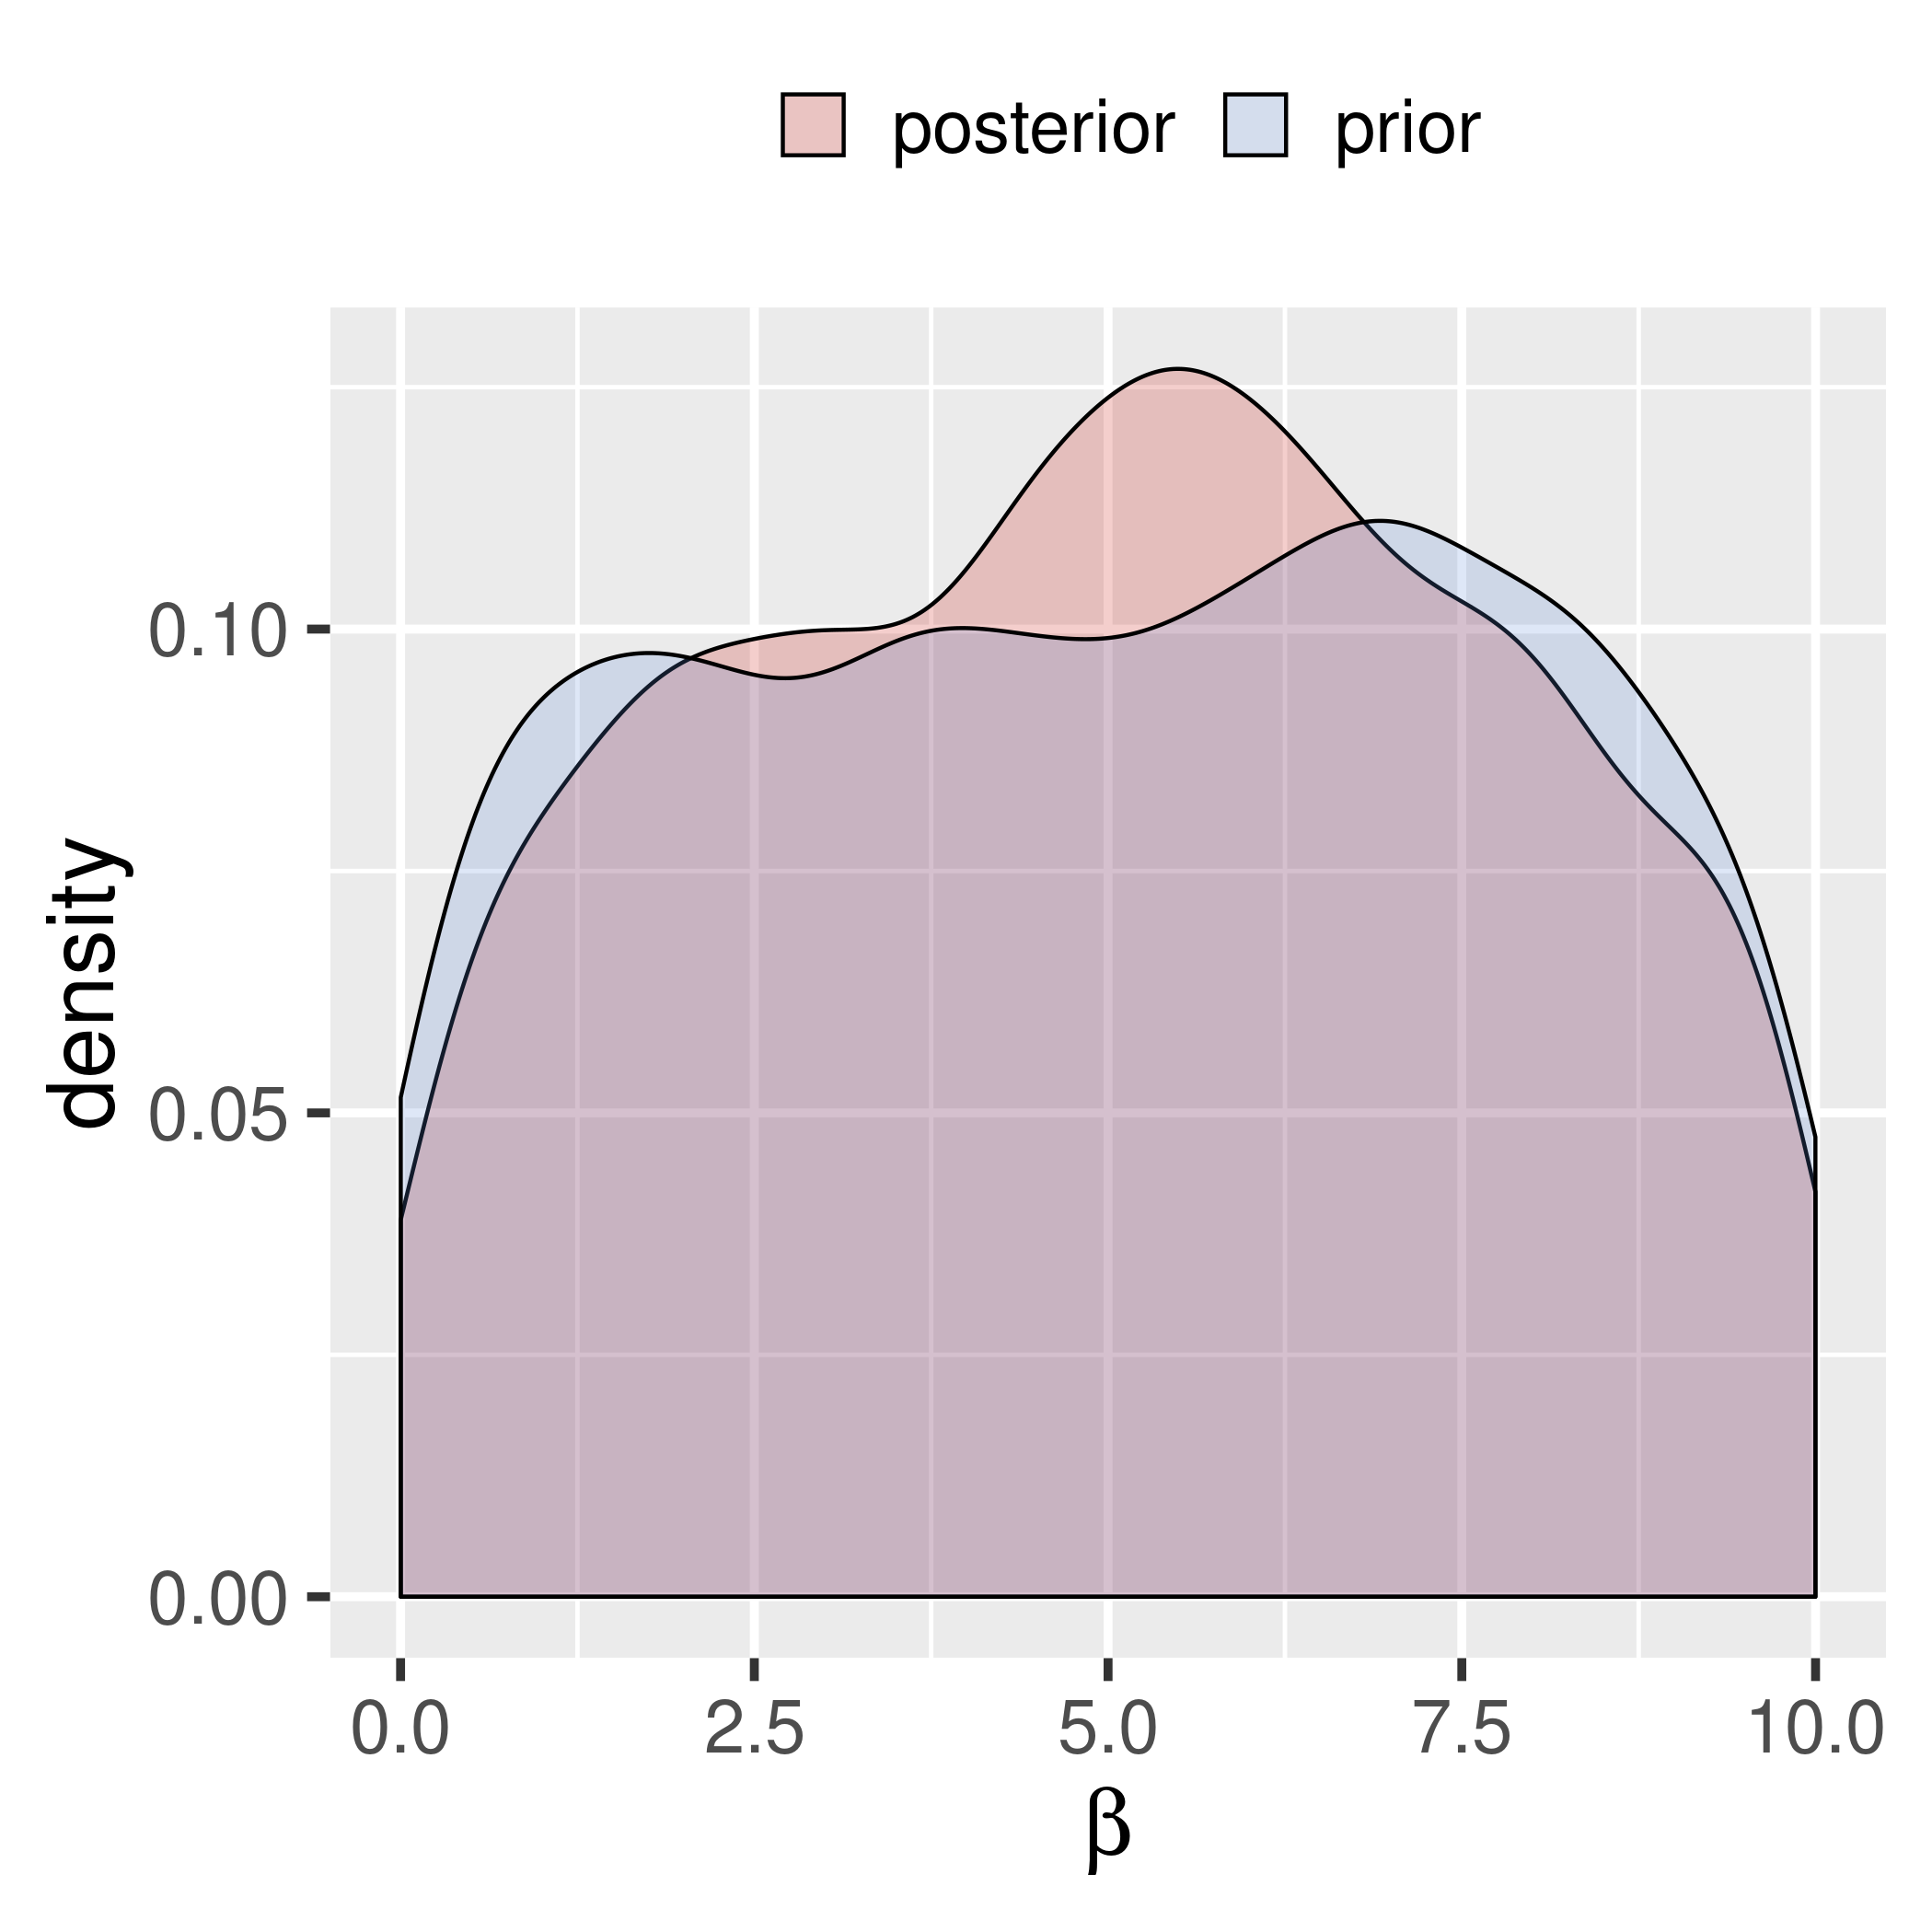
\includegraphics[width=0.6\textwidth]{van_allen_density_Q_beta.png}
    \caption{{\small Parameter $\beta$}}
    \label{fig:qbetavanAllen}
  \end{subfigure}
  \hfill
  \begin{subfigure}[b]{0.5\textwidth}
    \centering
    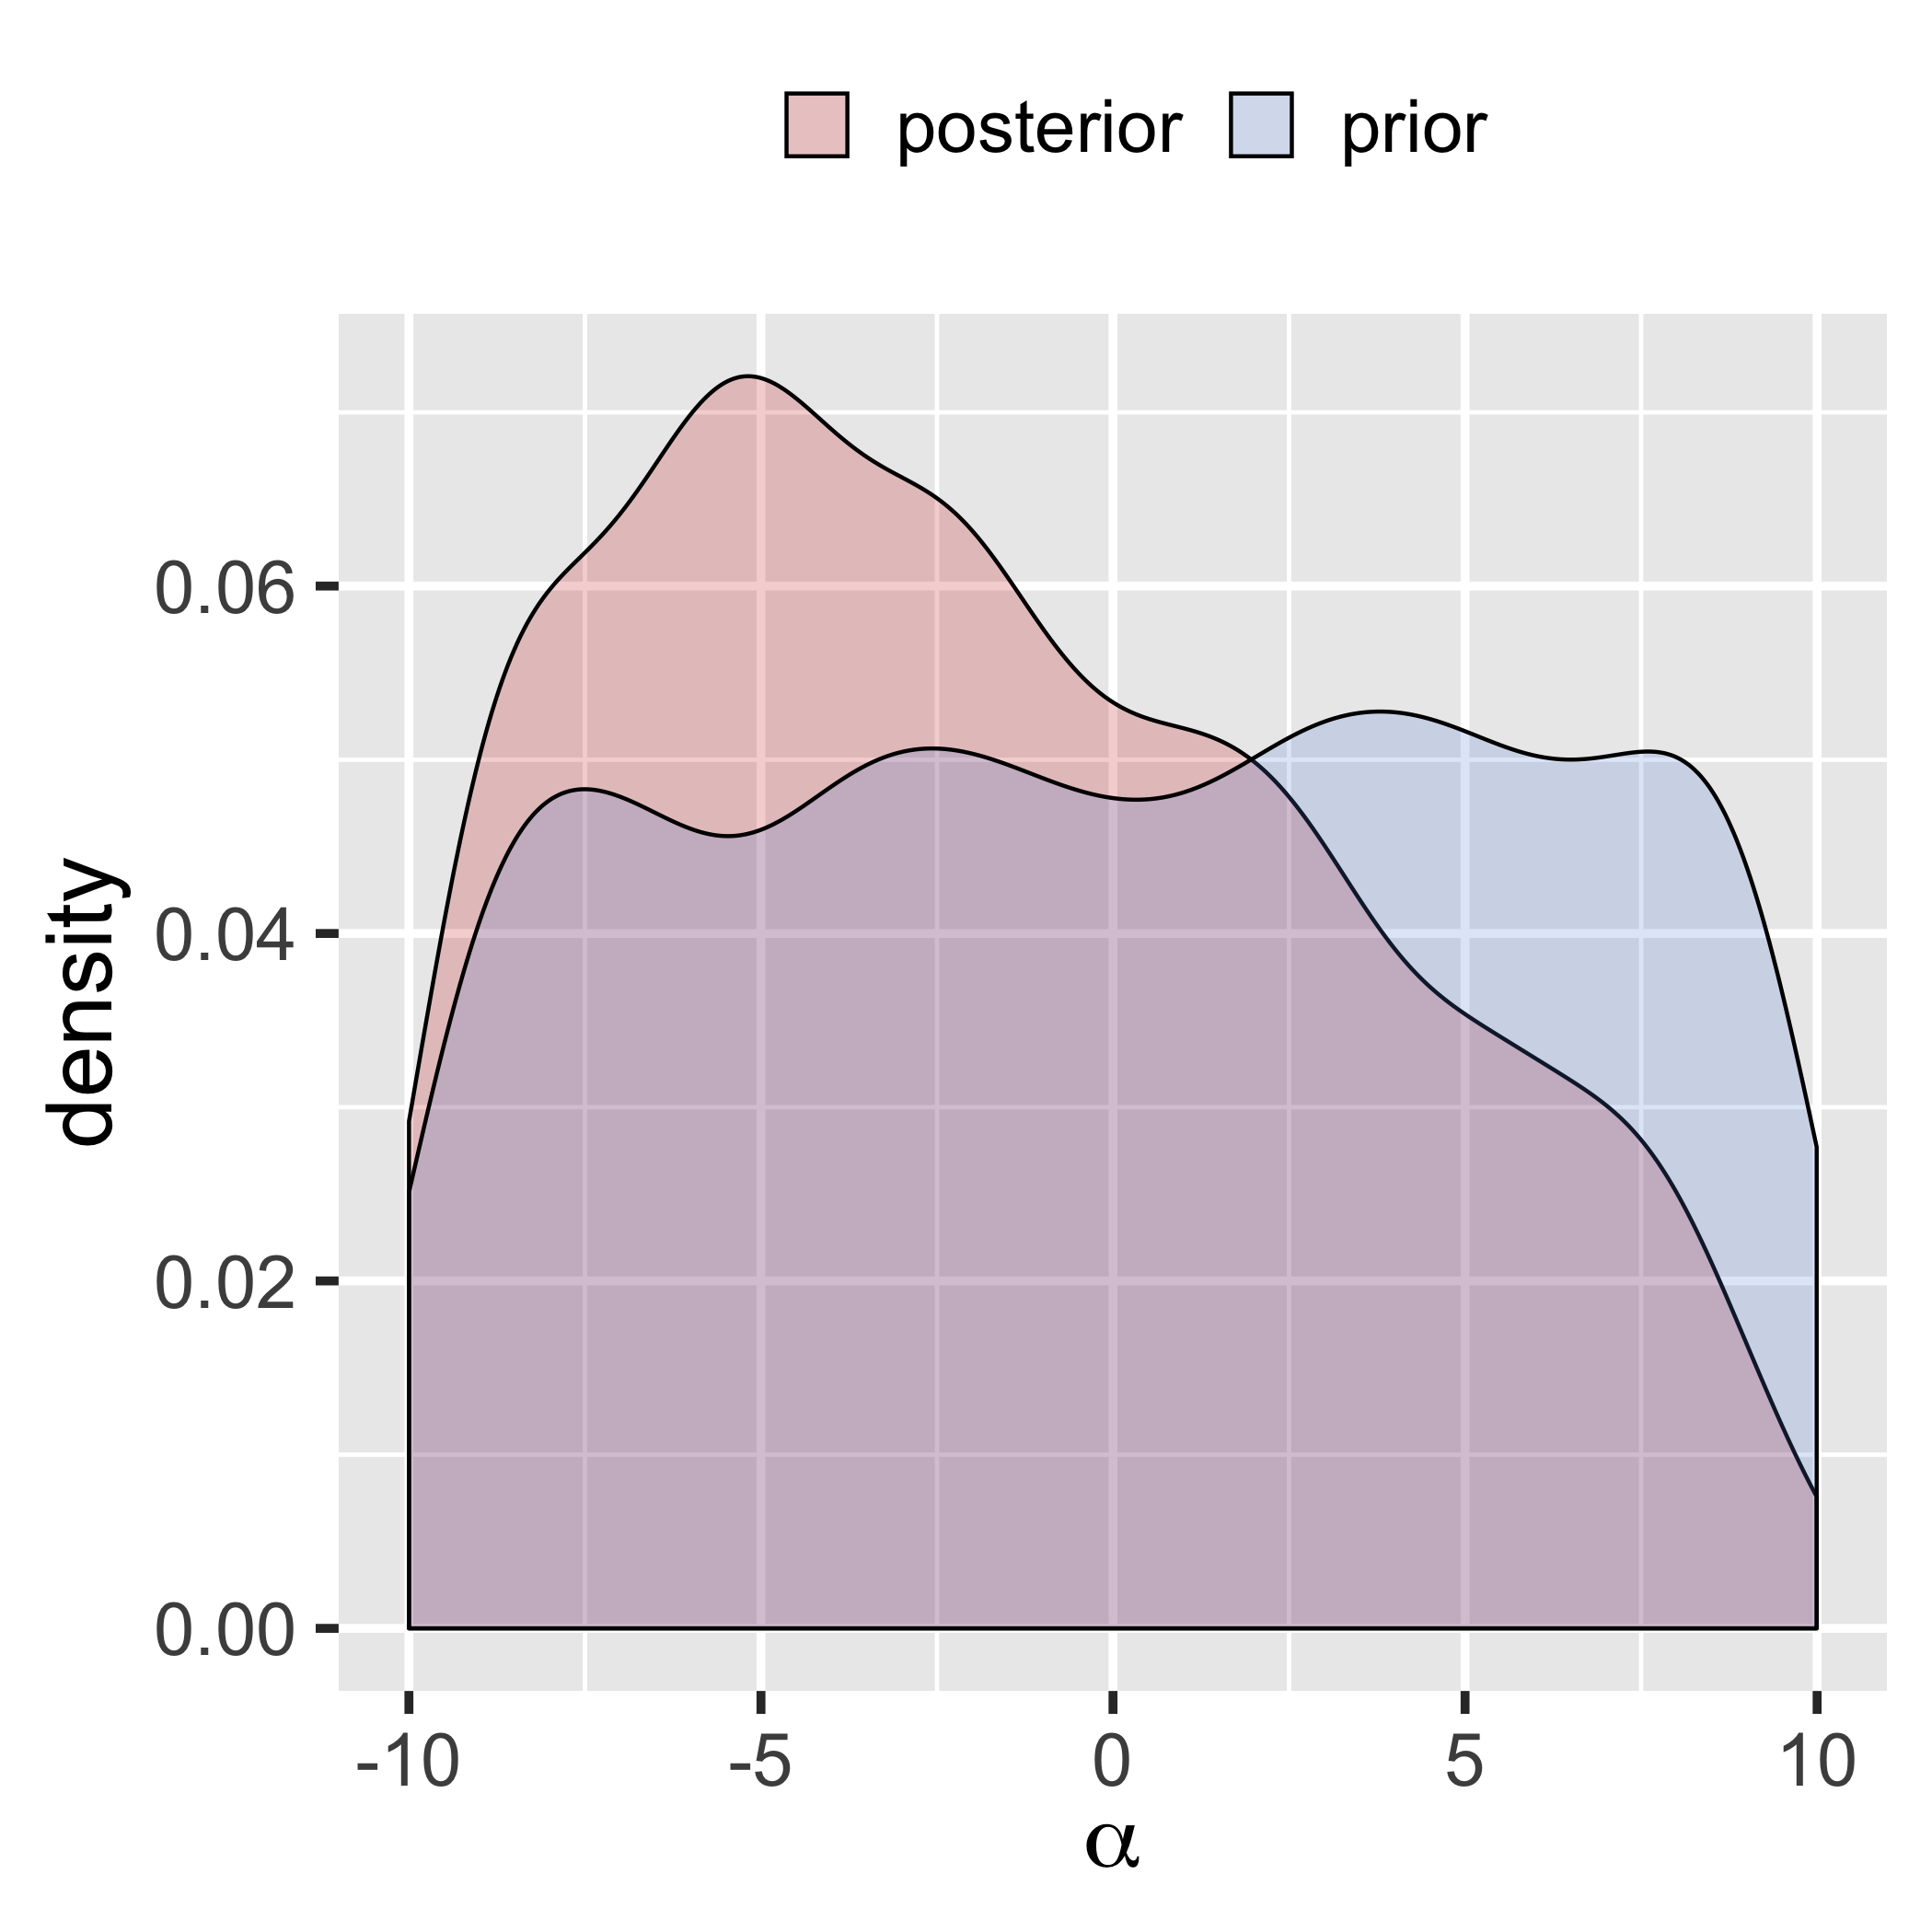
\includegraphics[width=0.6\textwidth]{van_allen_density_Q_alpha.png}
    \caption{{\small Parameter $\alpha$}}
    \label{fig:qalphavanAllen}
  \end{subfigure}
  \caption{
    \textbf{Van Allen Data}: Comparing prior and posterior densities 
    for the parameters of $q(\ell, t)$}  
\end{figure*}

\begin{figure*}[!htb]
  \centering
  \begin{subfigure}[b]{0.75\textwidth}
    \centering
    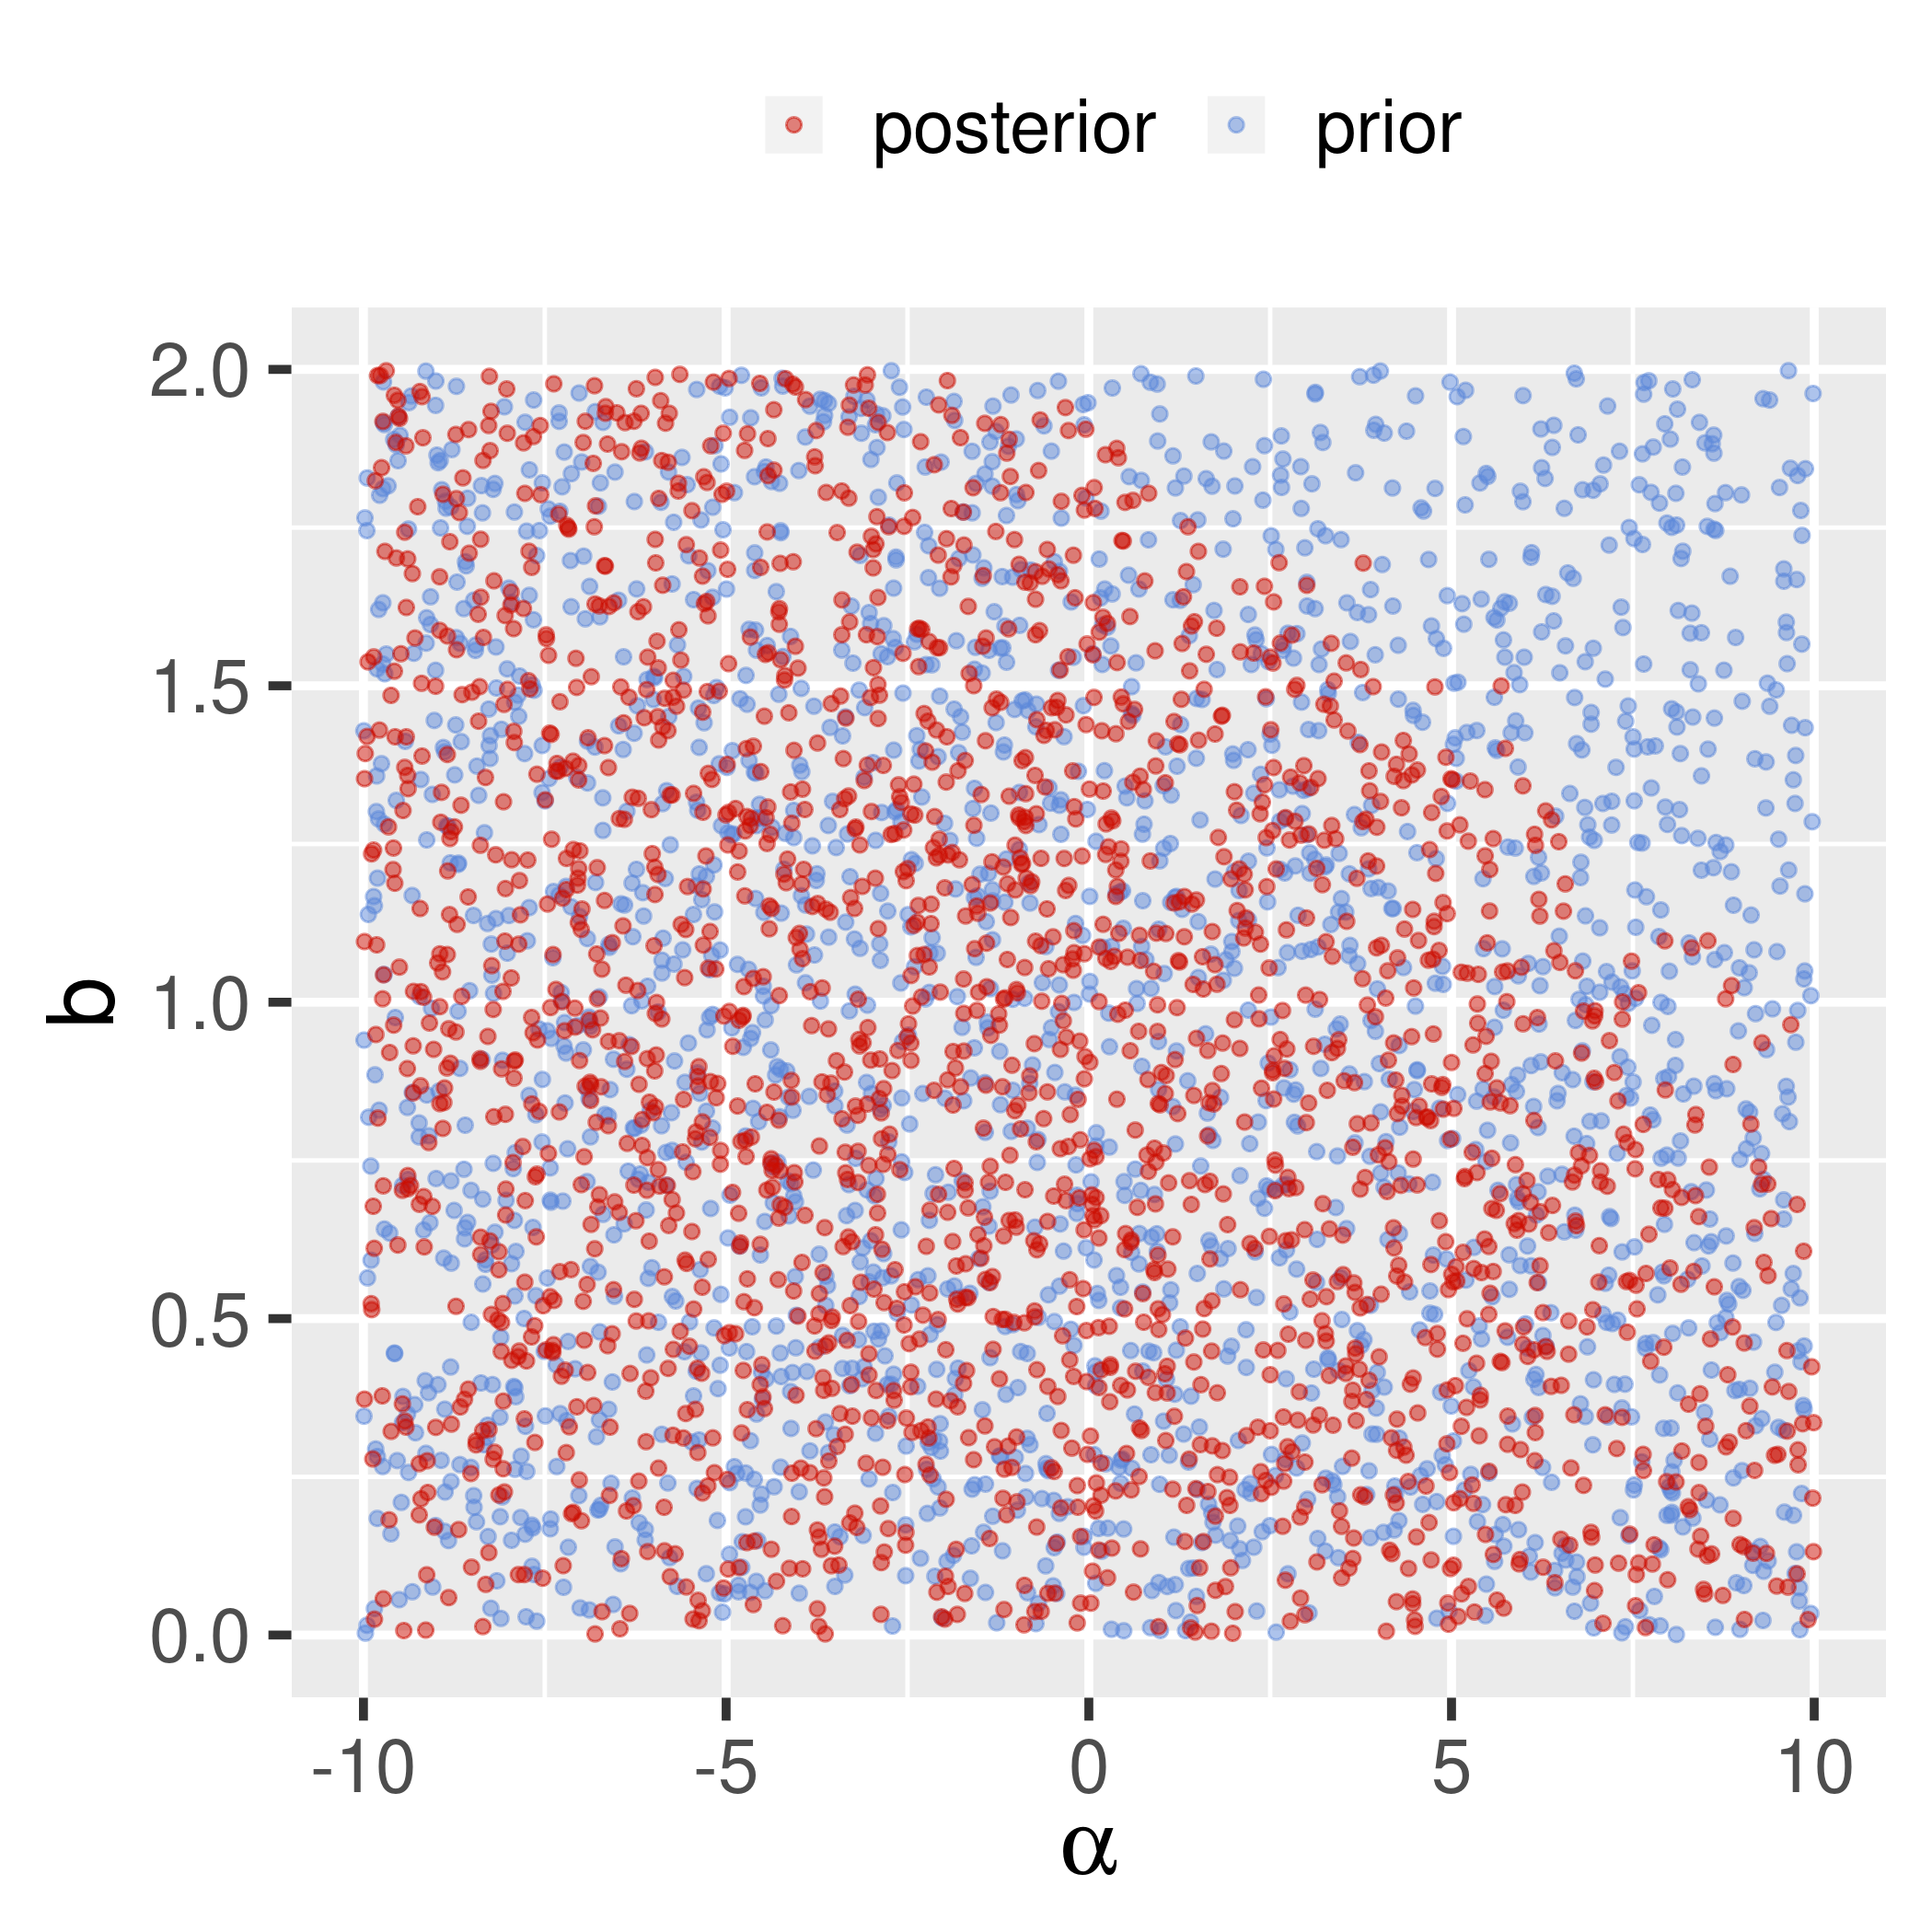
\includegraphics[width=0.6\textwidth]{van_allen_prior_posterior_scatter_Q_alpha_b.png}
    \caption{ 
      {\small Scatter chart: $\alpha$ versus $b$. } 
    }
    \label{fig:alphavsbvanAllen}
  \end{subfigure}
  \hfill
  \begin{subfigure}[b]{0.75\textwidth}
    \centering
    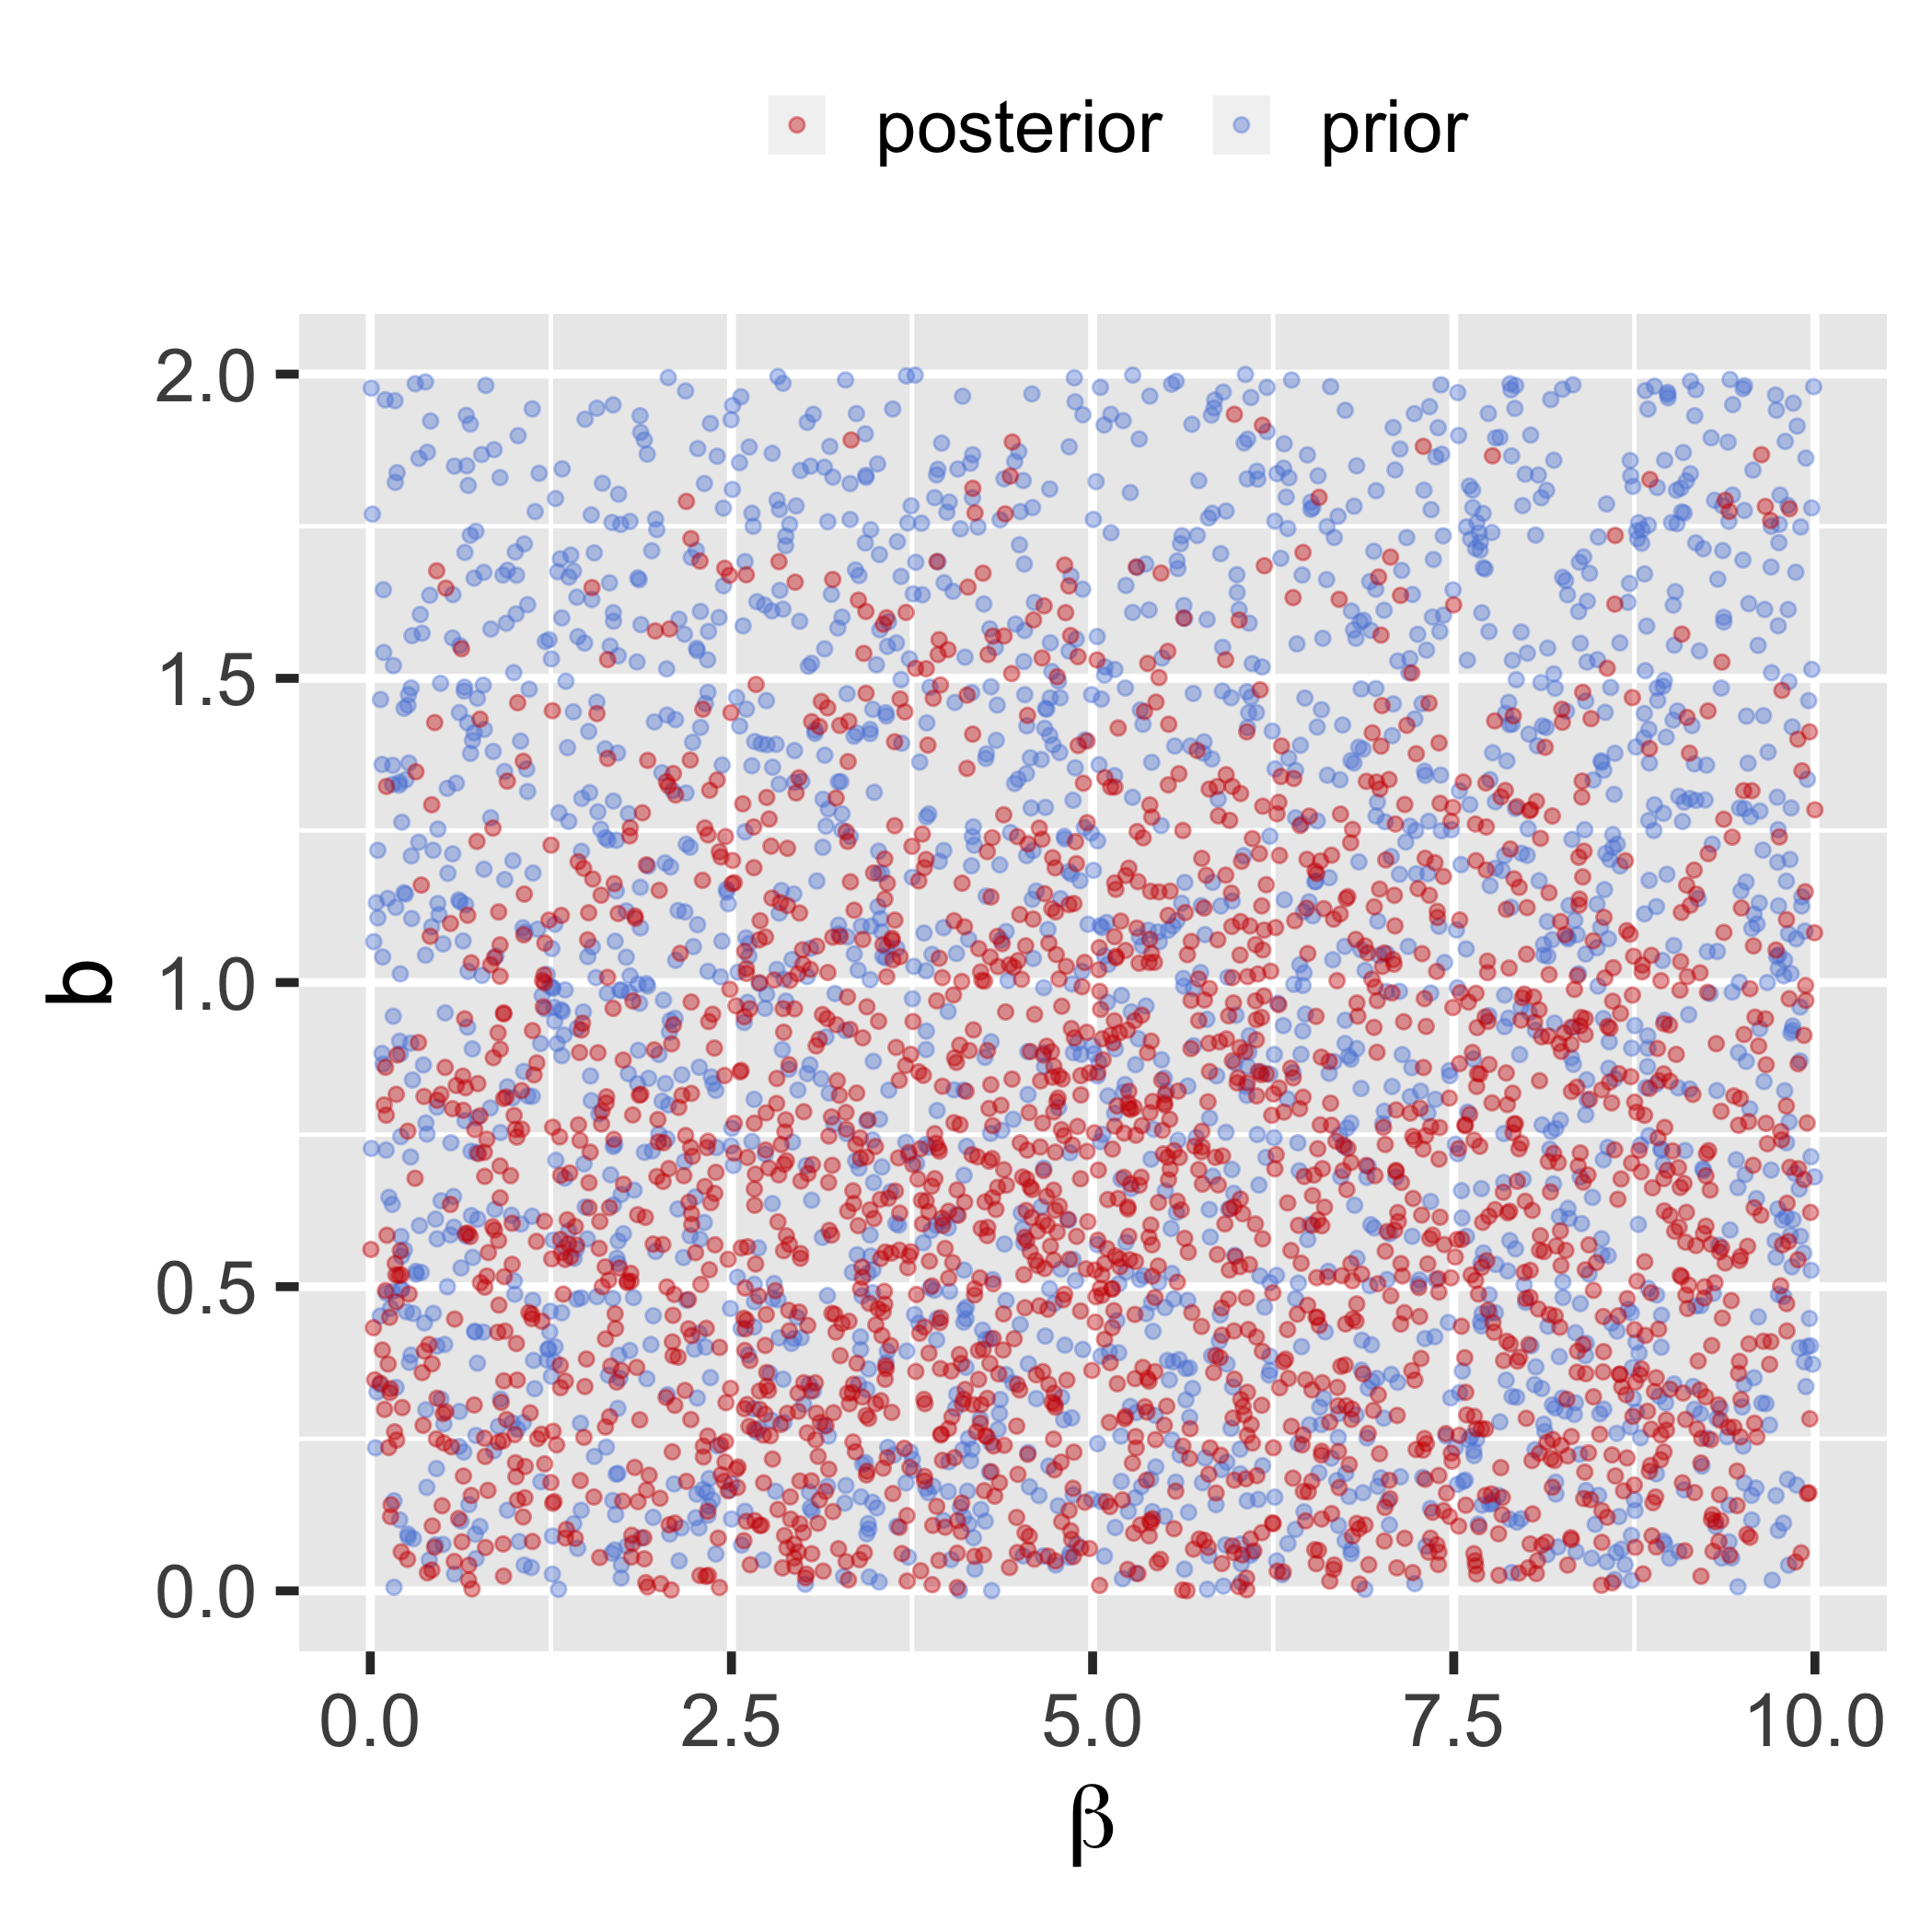
\includegraphics[width=0.6\textwidth]{van_allen_prior_posterior_scatter_Q_beta_b.png}
    \caption{
     {\small  Scatter chart: $\beta$ versus $b$.  }
    }
    \label{fig:betavsbvanAllen}
  \end{subfigure}
  \caption{
    \textbf{Van Allen Data}: Prior and posterior samples 
    drawn from parameters of $q(\ell, t)$.
  }
\end{figure*}
%\bibliographystyle{plainnat}
%\bibliography{references}
